\documentclass[12pt]{ucthesis}

\usepackage{etex}
\usepackage[morefloats=125]{morefloats}
\usepackage[hyphens]{url}
\usepackage[caption=false]{subfig}
\usepackage{graphicx}
\usepackage{tabularx}
\usepackage{amssymb}
\usepackage{amsmath}
\usepackage[letterpaper]{geometry}
\usepackage[overload]{textcase}
\usepackage{color}
\usepackage[nonumberlist,toc]{glossaries}
\usepackage{longtable}
\usepackage{threeparttablex} % for "ThreePartTable" environment
\usepackage{booktabs}        % for well-spaced horizontal rules
\usepackage{wrapfig}
\usepackage{longtable}
\usepackage{morefloats}
\usepackage{float}
\usepackage{listings}
\usepackage{makecell}
\usepackage{appendix}
\usepackage[]{algorithm2e}
\usepackage{titlesec}
\usepackage[breaklinks=true,hidelinks,pdfusetitle]{hyperref}
\usepackage{cleveref}
\usepackage{ifthen}
\usepackage{colortbl}
\usepackage{xcolor}
\usepackage{tikz}
\usetikzlibrary{tikzmark}

\setcounter{secnumdepth}{3}
\setcounter{tocdepth}{3}

% python listing
\lstset{language=Python}
\lstset{frame=lines}
\lstset{caption={Insert code directly in your document}}
\lstset{label={lst:code_direct}}
\lstset{basicstyle=\footnotesize}

% Added to avoid windows and orphans
\usepackage[all]{nowidow}
% Added to fix spacing between footnote entries
\usepackage{setspace}
\newlength{\myfootnotesep}
\setlength{\myfootnotesep}{\baselineskip}
\addtolength{\myfootnotesep}{-\footnotesep}
\setlength{\footnotesep}{\myfootnotesep} % set spacing between footnotes

\makeindex
\makeglossaries

% Shrink the size of headers
\titleformat{\chapter}[display]
        {\normalfont\normalsize\centering}
        {\ifthenelse{\equal{\thechapter}{A}}{APPENDICES\\[4.3ex]}{}\chaptertitlename\ \thechapter}
        {0pt}{\normalsize\uppercase}
\titlespacing*{\chapter}{0pt}{-20pt}{4.3ex plus .2ex}


\titleformat*{\section}{\normalsize\bfseries}
\titleformat*{\subsection}{\small\bfseries}
\titleformat*{\subsubsection}{\small\bfseries}
\titleformat*{\paragraph}{\small\bfseries}
\titleformat*{\subparagraph}{\small\bfseries}

\bibliographystyle{abbrv}

% Make \tindent indent pages if you have no paragraph indent
\newlength\tindent
\setlength{\tindent}{\parindent}
\setlength{\parindent}{0.in} \setlength{\parskip}{1.em}
\renewcommand{\indent}{\hspace*{\tindent}}
% Otherwise, comment out the above and uncomment this for default indentation on each paragraph
%\setlength{\parindent}{0.25in} \setlength{\parskip}{6pt}

\geometry{verbose,nohead,tmargin=1in,bmargin=1in,lmargin=1.5in,rmargin=1in}

% Different font in captions (single-spaced, bold) ------------
\newcommand{\captionfonts}{\small\bf\ssp}

\newcommand{\mycaption}[2]{\caption[#1 --- #2]{#1 --- #2}}

\makeatletter  % Allow the use of @ in command names
\long\def\@makecaption#1#2{%
  \vskip\abovecaptionskip
  \sbox\@tempboxa{{\captionfonts #1: #2}}%
  \ifdim \wd\@tempboxa >\hsize
    {\captionfonts #1: #2\par}
  \else
    \hbox to\hsize{\hfil\box\@tempboxa\hfil}%
  \fi
  \vskip\belowcaptionskip}
\makeatother   % Cancel the effect of \makeatletter
% ---------------------------------------

% Define Appendix refs
\crefname{app}{appendix}{appendices}
\Crefname{app}{Appendix}{Appendices}

% Add Figures folder to the graphics path
\graphicspath{{Figures/}{figures/}}

% Options for hyperref
\hypersetup{
    bookmarksnumbered=true,
    bookmarksopen=false,
    bookmarksopenlevel=0,
    colorlinks=false,
    pdfstartview=Fit,
    pdfborder={0 0 0},
}

\definecolor{dkgreen}{rgb}{0,0.6,0}
\definecolor{gray}{rgb}{0.5,0.5,0.5}
\definecolor{mauve}{rgb}{0.58,0,0.82}

\lstset{frame=tb,
  language=C++,
  aboveskip=3mm,
  belowskip=3mm,
  showstringspaces=false,
  columns=flexible,
  basicstyle={\small\ttfamily},
  numberstyle=\tiny\color{gray},
  keywordstyle=\color{blue},
  commentstyle=\color{dkgreen},
  stringstyle=\color{mauve},
  breaklines=true,
  breakatwhitespace=true,
  tabsize=2,
  numbers=left 
}

\newcounter{qcounter}
\providecommand{\keywords}[1]{\textbf{\textit{Keywords:}} #1}


\begin{document}

% Declarations for Front Matter
\title{Scalable Cognitive Radio Network Testbed in Real Time}
\author{Kevin Zhipeng Yu}
\degreemonth{June} \degreeyear{2021} \degree{Master of Science}
\defensemonth{June} \defenseyear{2021}
\numberofmembers{3}
   \chair{Tina Smilkstein, Ph.D. \linebreak Associate Professor of Electrical Engineering}
   \othermemberA{Hugh M. Smith, Ph.D. \linebreak Professor of Computer Science}
   \othermemberB{Jason Peters, Ph.D. \linebreak Assistant Professor of English}
\field{Electrical Engineering} \campus{San Luis Obispo}
\field{Computer Science} \campus{San Luis Obispo}
\field{English} \campus{San Luis Obispo}
\copyrightyears{seven}


\maketitle

\begin{frontmatter}

% Custom made for Cal Poly (by Mark Barry, modified by Andrew Tsui).
\copyrightpage

% Custom made for Cal Poly (by Andrew Tsui).
\committeemembershippage

\begin{abstract}
Modern society places an increasingly high demand on data transmission. Much of that data transmission takes place through communication over the frequency spectrum. The channels on the spectrum are limited resources. Researchers realize that at certain times of day some channels are overloaded, while others are not being fully utilized. A spectrum management system may be beneficial to remedy this efficiency issue. One of the proposed systems, Cognitive Radio Network (CRN), has progressed over the years thanks to studies on a wide range of subjects, including geolocation, data throughput rate, and channel handoff selection algorithm, which provide fundamental support for the spectrum management system. To move CRN technology forward, in this thesis we propose a physical, scalable testbed for some of the extant CRN methodologies. This testbed integrates IEEE standards, FCC guidelines, and other TV band regulations to emulate CRN in real time. With careful component selections, we include sufficient operational functionalities in the system, while at the same time making sure it remains affordable. We evaluate the technical feasibility of the testbed by studying several simple CRN logics. When comparing a system with a selection table implemented to those with na\"ive selection methods, there is more than a 60 percent improvement in the overall performance.

\end{abstract}

\begin{acknowledgements}
\noindent
First, I would like to give thanks to my parents who supported me through this tough time this past year. They work so hard in exchange for my accomplishments in school. Their love and care toward me is invaluable and ineffable.

Next, I want to show my most gratitude to all my committees. Professor Smilkstein inspired and guided me through every detail of the thesis. Over the course, I give credit to her who instructed and advised with insights on related topics. I appreciated the intentionality from Professor Smith. It was him who taught Network with passion, which motivated me to take a step further with this project. Special thanks to Dr. Peters in the College of Liberal Art. I am grateful to have him, being a non-technical audience, advising me on the thesis report. Each of my committees assist me in ways that are most helpful. Thank you. 

Lastly, I also would like to thank all the tutors who helped me at the Cal Poly "Writing and Learning Initiatives" program. And, I give thanks to my roommate Charlie who helped me solder all the components in a timely manner. 




\end{acknowledgements}

\tableofcontents

\listoftables

\listoffigures

% \lstlistoflistings

% Add CHAPTER into table of contents.
\addtocontents{toc}{%
   \noindent CHAPTER
}

\end{frontmatter}

\pagestyle{plain}

\renewcommand{\baselinestretch}{1.66}

\chapter{Introduction}

Data is transmitted everywhere in the air around us. As the data demand gets larger each year, engineers make use of all of the different 
channels and bands. People these days discover that the transmission channels are in fact limited. In many countries, there is an administrative
agency which regulates the band allocation. Here in United States, the National Telecommunications and Information Administration 
(NTIA) and the Federal Communications Commission (FCC) are responsible for allocating bands for government, organizational and
individual uses. A licensed band user is given a range of frequency in the spectrum where they can freely utilize data transmission
in the air. However, recent studies report, at certain frequencies (bands), there is only a low 15 percent of utilization, where other
channels were overwhelming with data crossing. This creates large load distribution gaps as shown in Figure~\ref{fig:spectrum_utilization}.

\begin{figure}[ht]
\centering
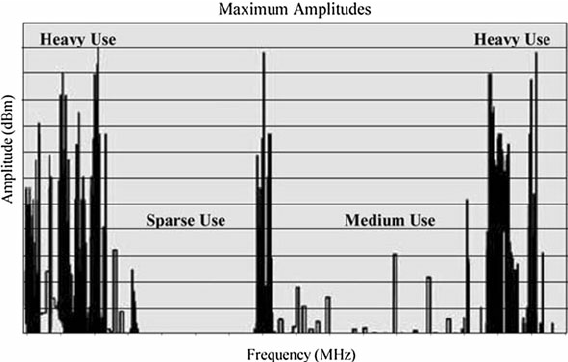
\includegraphics[width=12cm]{figures/spectrum_utilization.png}
\caption{Spectrum Utilization \cite{improved_local}}
\label{fig:spectrum_utilization}
\end{figure}

It is possible to balance the load across the whole spectrum. By keeping this objective in mind, scientists have proposed spectrum 
management solutions year to year; one of these solutions is using Cognitive Radio (CR). CR is under the category of Software Defined Radio 
(SDR), which is programmable and adaptive to varying complex environment \cite{software_defined_radio}. Regarding the topic of Cognitive Radio Network (CRN), it is still a broad, ongoing research project. One area that people research for is optimizing the channel utilization. They generally looking for the best channel handoff algorithm to avoid more "holes" in the channel shown in Figure~\ref{fig:channel_hole}. A good handoff algorithm can fill in much of the holes during the transmission process. This directly improve the spectrum utilization. Many related papers claim to have a 
more efficient algorithm compared to others, more specifically, they are looking at the effects of different channel 
selection algorithms. A two phase real-time spectrum handoff algorithm that Chakraborty and Misra propose in their conference paper confirms a 40 to 60 percent decrease in spectrum handoff delay in simulation models \cite{real_time_spectrum}. Analytically, it has a minimum 10 percent reduction in Voice over IP (VoIP) call-dropping probability. In Varade and Ravinder's paper, in simulation, they show their Genetic Algorithm (GA) resulting a overall efficiency of 94 percent of fitness measures by optimizing transmission parameters \cite{optimal_spectrum_allocation}.

\begin{figure}[ht]
\centering
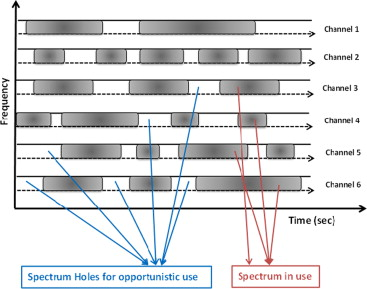
\includegraphics[width=12cm]{figures/channel_hole.jpg}
\caption{Spectrum Utilization \cite{idle_channel}}
\label{fig:channel_hole}
\end{figure}

This thesis project contributes to the field by compiling an emulator that composes scalable software integration and accessible
hardware for the CRN. Notice not many paper under the area actually deploy hardware to test their program for the network 
With all those intelligent channel selection algorithms from proposers, testing them at real time should essentially be the 
next step. Yet, they hesitate to move forward, one reason is because we do expect a significant spending on the setup of the physical 
testing environment. Before the full development of a specific hardware for systematic testing are put into action, a general purposed testbed 
can make it easier to validate any functional characteristic with proposed algorithm. 
A desire physical testbed can adapt to different program and stimulus. Ultimately, it records and return meaningful data that entail the performance of the system under test.

Using the thesis project emulator framework for real time experiment, to a good extent, one can estimate the performance of a channel 
selection algorithm. It costs well under \$50 for the whole system. If experiment run time is an issue, one can adjust
the timing ratio to minimize the uses of resource. Despite of its simplicity, the implementation follows closely to IEEE
standard and FCC guildline.

To understand the significant of the project, the thesis paper first explains some of the background of the technology in Chapter 2.
Chapter 3 describes the design choices during software development. Chapter 4 illustrates physical modules and a fine prototype.
To test the usability of the system, the project included a performance comparison of a channel selection method with history table and in-order/random selection in Chapter 5. Last chapter, Chapter 6 concludes the work and discuss its future possible route. 





\chapter{Background}
\section{Working Principle}

Every type of wireless data transmission only transmits in a designated frequency. It would get crowded in the air when many users 
are on a single channel. Think about traffic on the highway, there should be multiple lanes designated for different purposes. 
All the vehicles drive on their lane based on the rule. You have roadways, passing lanes, carpool lanes, emergency lanes, etc. 
It will get very crowded on the roadways during certain times of the day due to high volume of cars, where less or no one is 
using any of the carpool lanes or emergency lanes. This occurs in wireless communication, too. Different channels or frequencies
are assigned to different public organizations, private sectors or other stations. 
During certain times of the day, people use their typical devices, which may transmit data only on a designated channel.
This is the same situation as traffic is all crowded in one lane. Integrating a cognitive radio network is basically adding a traffic light or employing highway patrol for the busy channels. When primary users are not using their license band, they are considered open channels. If the no one do anything to it, this results in very low utilization. The main idea for Cognitive Radio Network is to create
a smart networking environment for a secondary user (SU) to use those idle bands. SU is free to use the band as long as the 
primary user (PU) is not here. When the PU of the band comes, SU must handoff to another band that is free. Generally, using
such handoff mechanism, it increases the spectrum utilization overall. 


\section{Application}

One utilization of the cross channels transmission mechanism enables a way to implement Internet of Things (IoT), which means
everything in life can share their obtained knowledge with everything else. 
IoT helps automated machines to make better 
decisions in real time. IEEE standard 802.22.3, or now transiting to 802.15, has designated working groups in IoT area
\cite{ieee_working_group}. Electric devices like smart refrigerator, smart fan, or smart lamp is mostly connected online
using WiFi or Zigbee technology. The transmission load will eventually overwhelm both spectrum ranges as the devices scale
up. With cognitive radio technology, it will help release some of the stress from these bands.

Because of the nature of the radio frequency that CR uses, it also can be applied very well at sub-urban areas and big cities.
In theory, it can transmit as far as 100 kilo-meter range as Figure~\ref{fig:radio_range} demonstrates. These numerical values are obtained from IEEE standards and their specification. The only drawback
is, even as the signal is traveling at the speed of light, it inevitably has minor delay for every transmission. For those
applications that put latency metric as least priority, that wouldn't be an issue. It can still work well with essential
rural communication, traffic division, emergency broadcast, etc. 


\begin{figure}[ht]
\centering
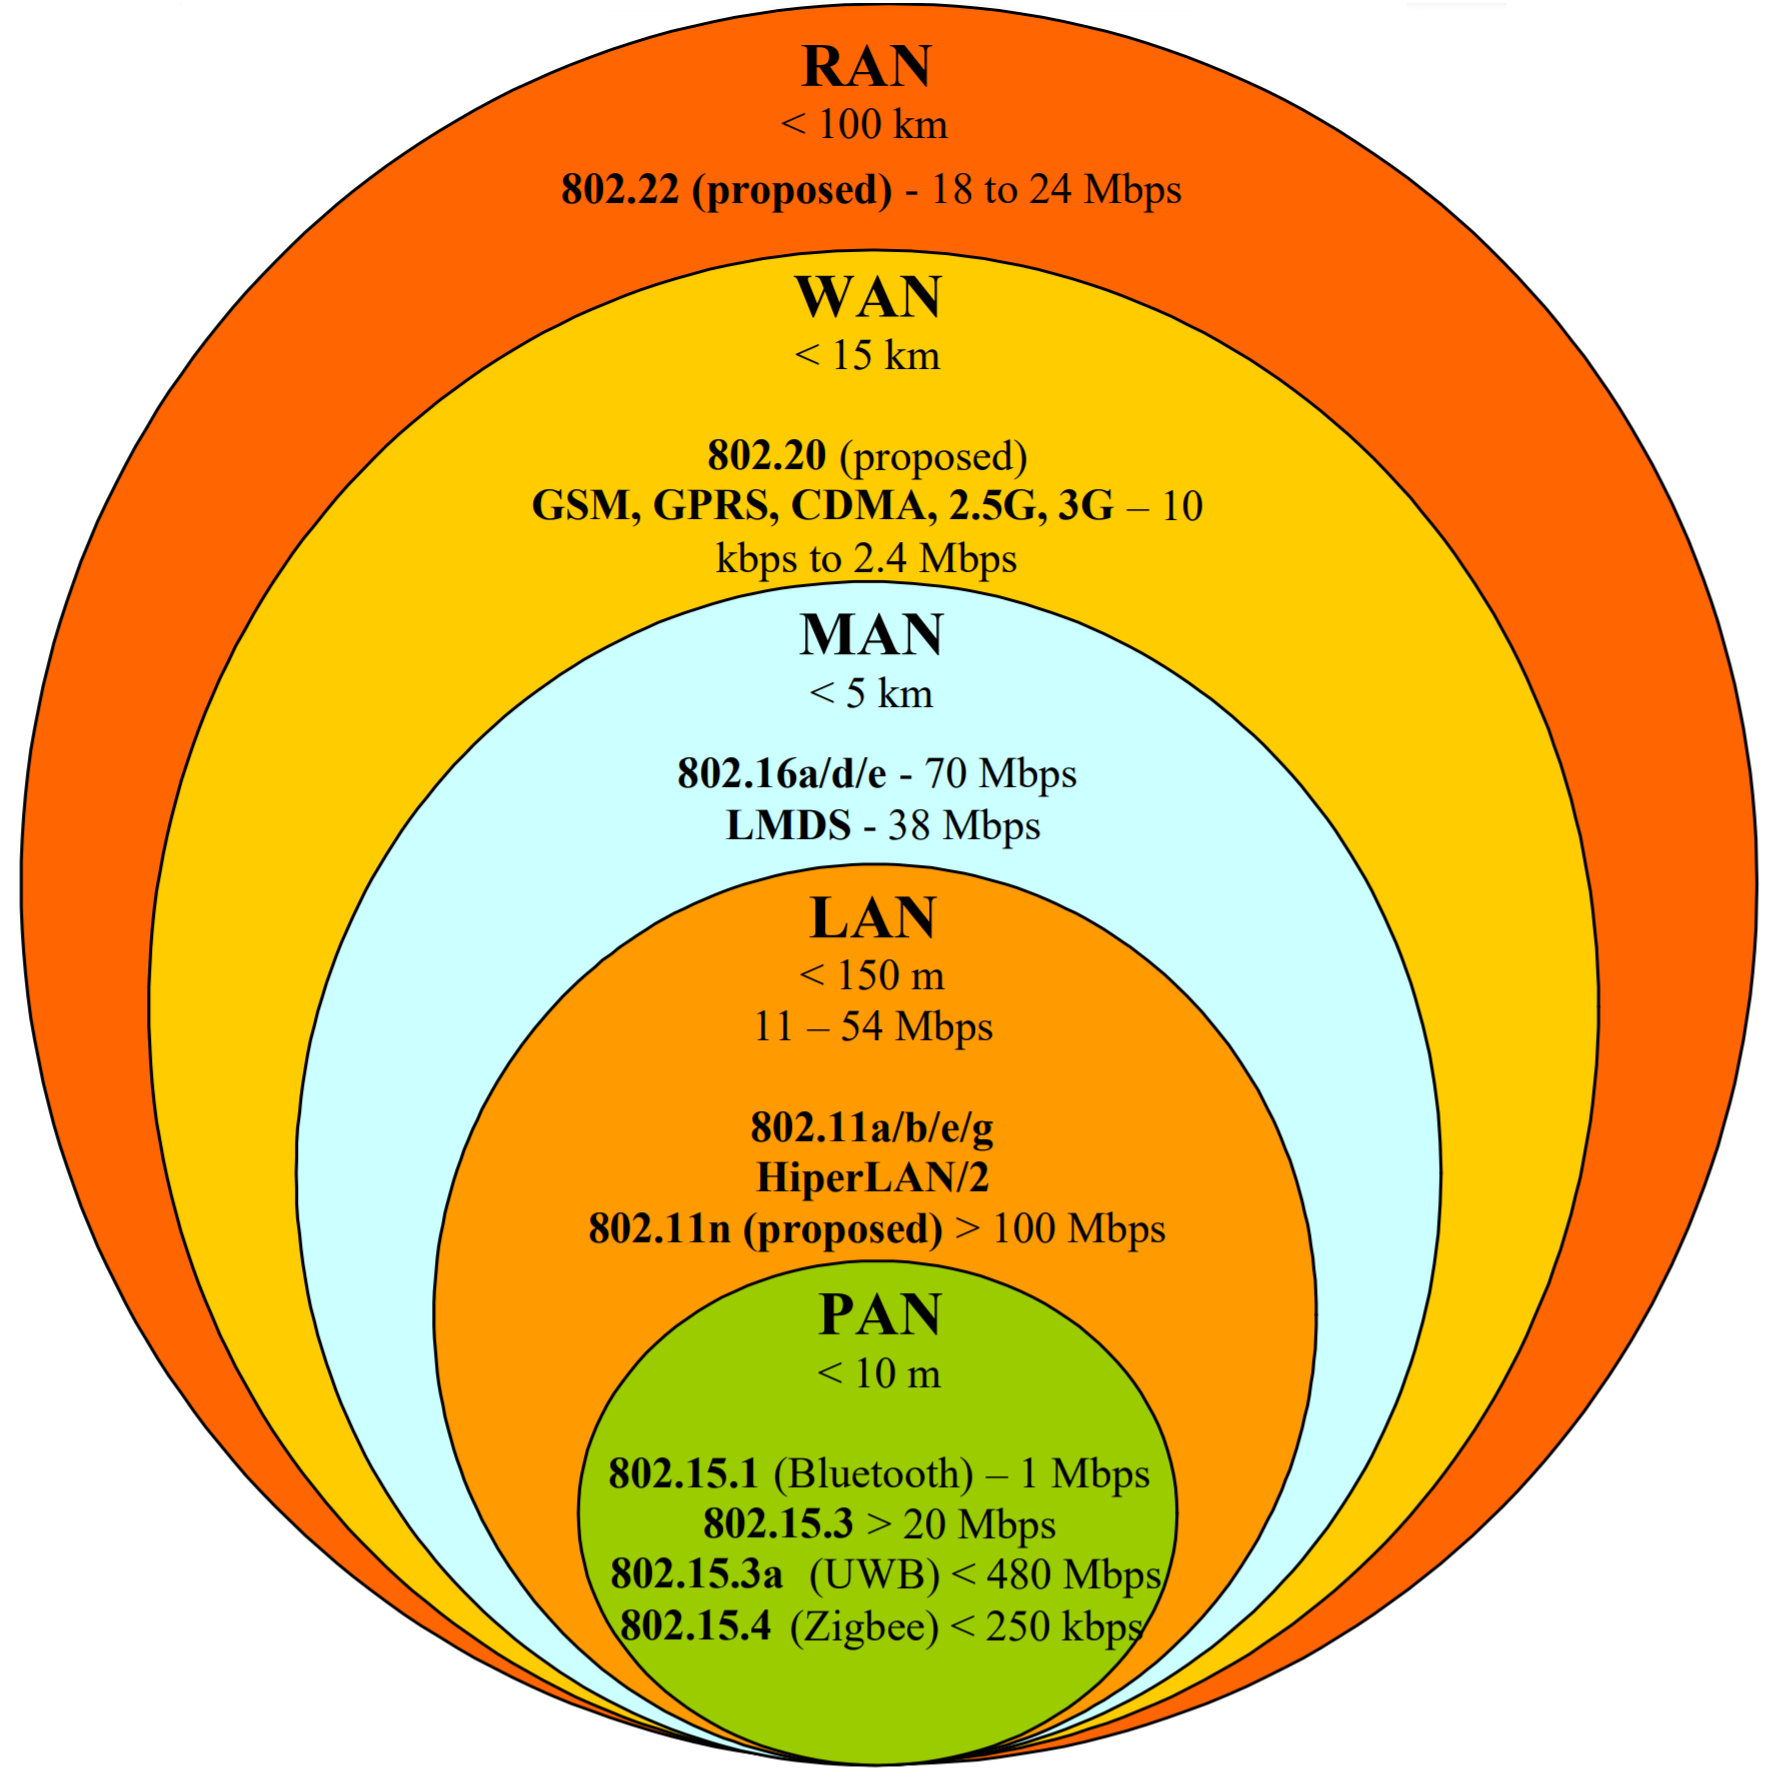
\includegraphics[width=10cm]{figures/radio_range.png}
\caption{Radio Standard Range \cite{ieee_802_22}}
\label{fig:radio_range}
\end{figure}

Continuing the topic of CRN limitation, disturbance is another concern for the licensed band users. Due to imperfection of
the CR system, during PU operation hours, if another SU is also transmitting, it would be considered as noise to the 
primary services. PU would like to discourage such technology if any of these interruptions happen frequently. However, during non-operation hours, the band owners could sub-lease their bands to anyone who uses CR. This potentially bring a
market and demand of the shareable network.

\section{History}
After discussing so much of the application opportunity of the CRN, let's revisit the history of the technology with 
more appreciation. The idea of cognitive radio was first introduced by Joseph Mitola III at KTH in 1998. It sounded 
merely just another idea to organize the band usage. People knew this is a way to maximize band utilization after all.
Not long after that, in the year 2000, there was a huge explosion in a Netherlands firework factory \cite{cr_history}. 
23 people were killed. Local emergency hotlines faced serious communication issue during the crisis which lead to further
deterioration and destruction. This same problem happened during 9/11 in the United States in 2001. These incidents
pushed intellectual and academic societies to work towards developing a better management system for the electromagnetic
spectrum. People realize CR is not just a tool help setting up extra communication channel when under load, it
potentially open up emergency lines to save lives. With higher precaution awareness and a rising demand on data usage, such as IoT applications, in our time, managing the frequencies properly is the top priority. With the goals and current technology, scientists and engineers
begin to work on different areas relating to optimizing and setting up the network.

The first cognitive radio standard IEEE 802.22 was published by IEEE 802 LAN/MAN Standard Committee (LMSC)in 2011. 
IEEE 802 Part 22 also known as Wireless Regional Area Networks (WRAN) standard. It specified geolocation and spectrum
sensing methodology. Geolocation relies on a databases composed of licensed transmitters in the area and geographical 
realm for the CRN. For a CR device, each is capable of sensing the channel status (busy or idle). It also needs to be 
capable of sensing the source of the frequency in the air. Spectrum sensing often utilize one of the following, energy 
detector, matched filter, cyclostationary process. Energy detection is by far the most used way in radio-frequency 
integrated circuit (RFIC) chips. 


\section{Characteristics}
IEEE 802 Part 22 states an entire regulation on the policies and procedures for operating in the TV bands. 
Table~\ref{tab:physical} summarize the key points in the Physical Layer (PHY) specifications. For TV bands, 
the transmit frequency in the air generally set between at the very high frequency (VHF) and the ultra high frequency (UHF) range
for quality and long distance data transmission. Depends on the regions, channel bandwidth can be varied which lead to
different throughput values. The overall throughput of the data flow can go up to 22.69 Mbit per second.
The modulation method can adapt to the most usable technology at the current time and space. 


\begin{table}[ht]
\centering
\setlength{\tabcolsep}{20pt}
\renewcommand{\arraystretch}{1.5}
\begin{tabular}{| l | l |}
\hline
\hspace{0.3cm}  Environment & TV broadcast white space \\ 
\hline
\hspace{0.3cm}  Frequency range &  54 - 862 MHz  (VHF - UHF)\\ 
\hline
\hspace{0.3cm}  Channel bandwidth &  6, 7 or 8 MHz \\ 
\hline
\hspace{0.3cm}  Throughput &  4.54 - 22.69 Mbs  \\ 
\hline
\hspace{0.3cm}  Modulation &  QPSK, 16-QAM or 64-QAM  \\ \hline
\hline
\end{tabular}
\caption{Physical Layer Characteristics}
\label{tab:physical}
\end{table}

Moving on to the Cognitive WRAN Medium Access Control (MAC) specifications. As states in IEEE 802.22, devices should have 48
bits MAC address for identification in the net. Connections between devices should also have 12 bits Company Identifier (CID). The 
connections are assembled with a stream of data, called superframe. A superframe is constructed of a preamble, synchronize channel (SCH) and 16 frames
in total. Figure~\ref{fig:frame} shows the transmission through a time period and the frame structure at a couple of the opened channels in the TV band. The red bars across time indicate there are occupations to the TV channels at the specific frequencies. Yet, the system shown should spot the idle channels in the middle at around some frequency of t. And it begins the channel synchronization process by sending preamble and SCH to the channel. After it is in sync, secondary devices can exchange data in the frames. 

\begin{figure}[ht]
\centering
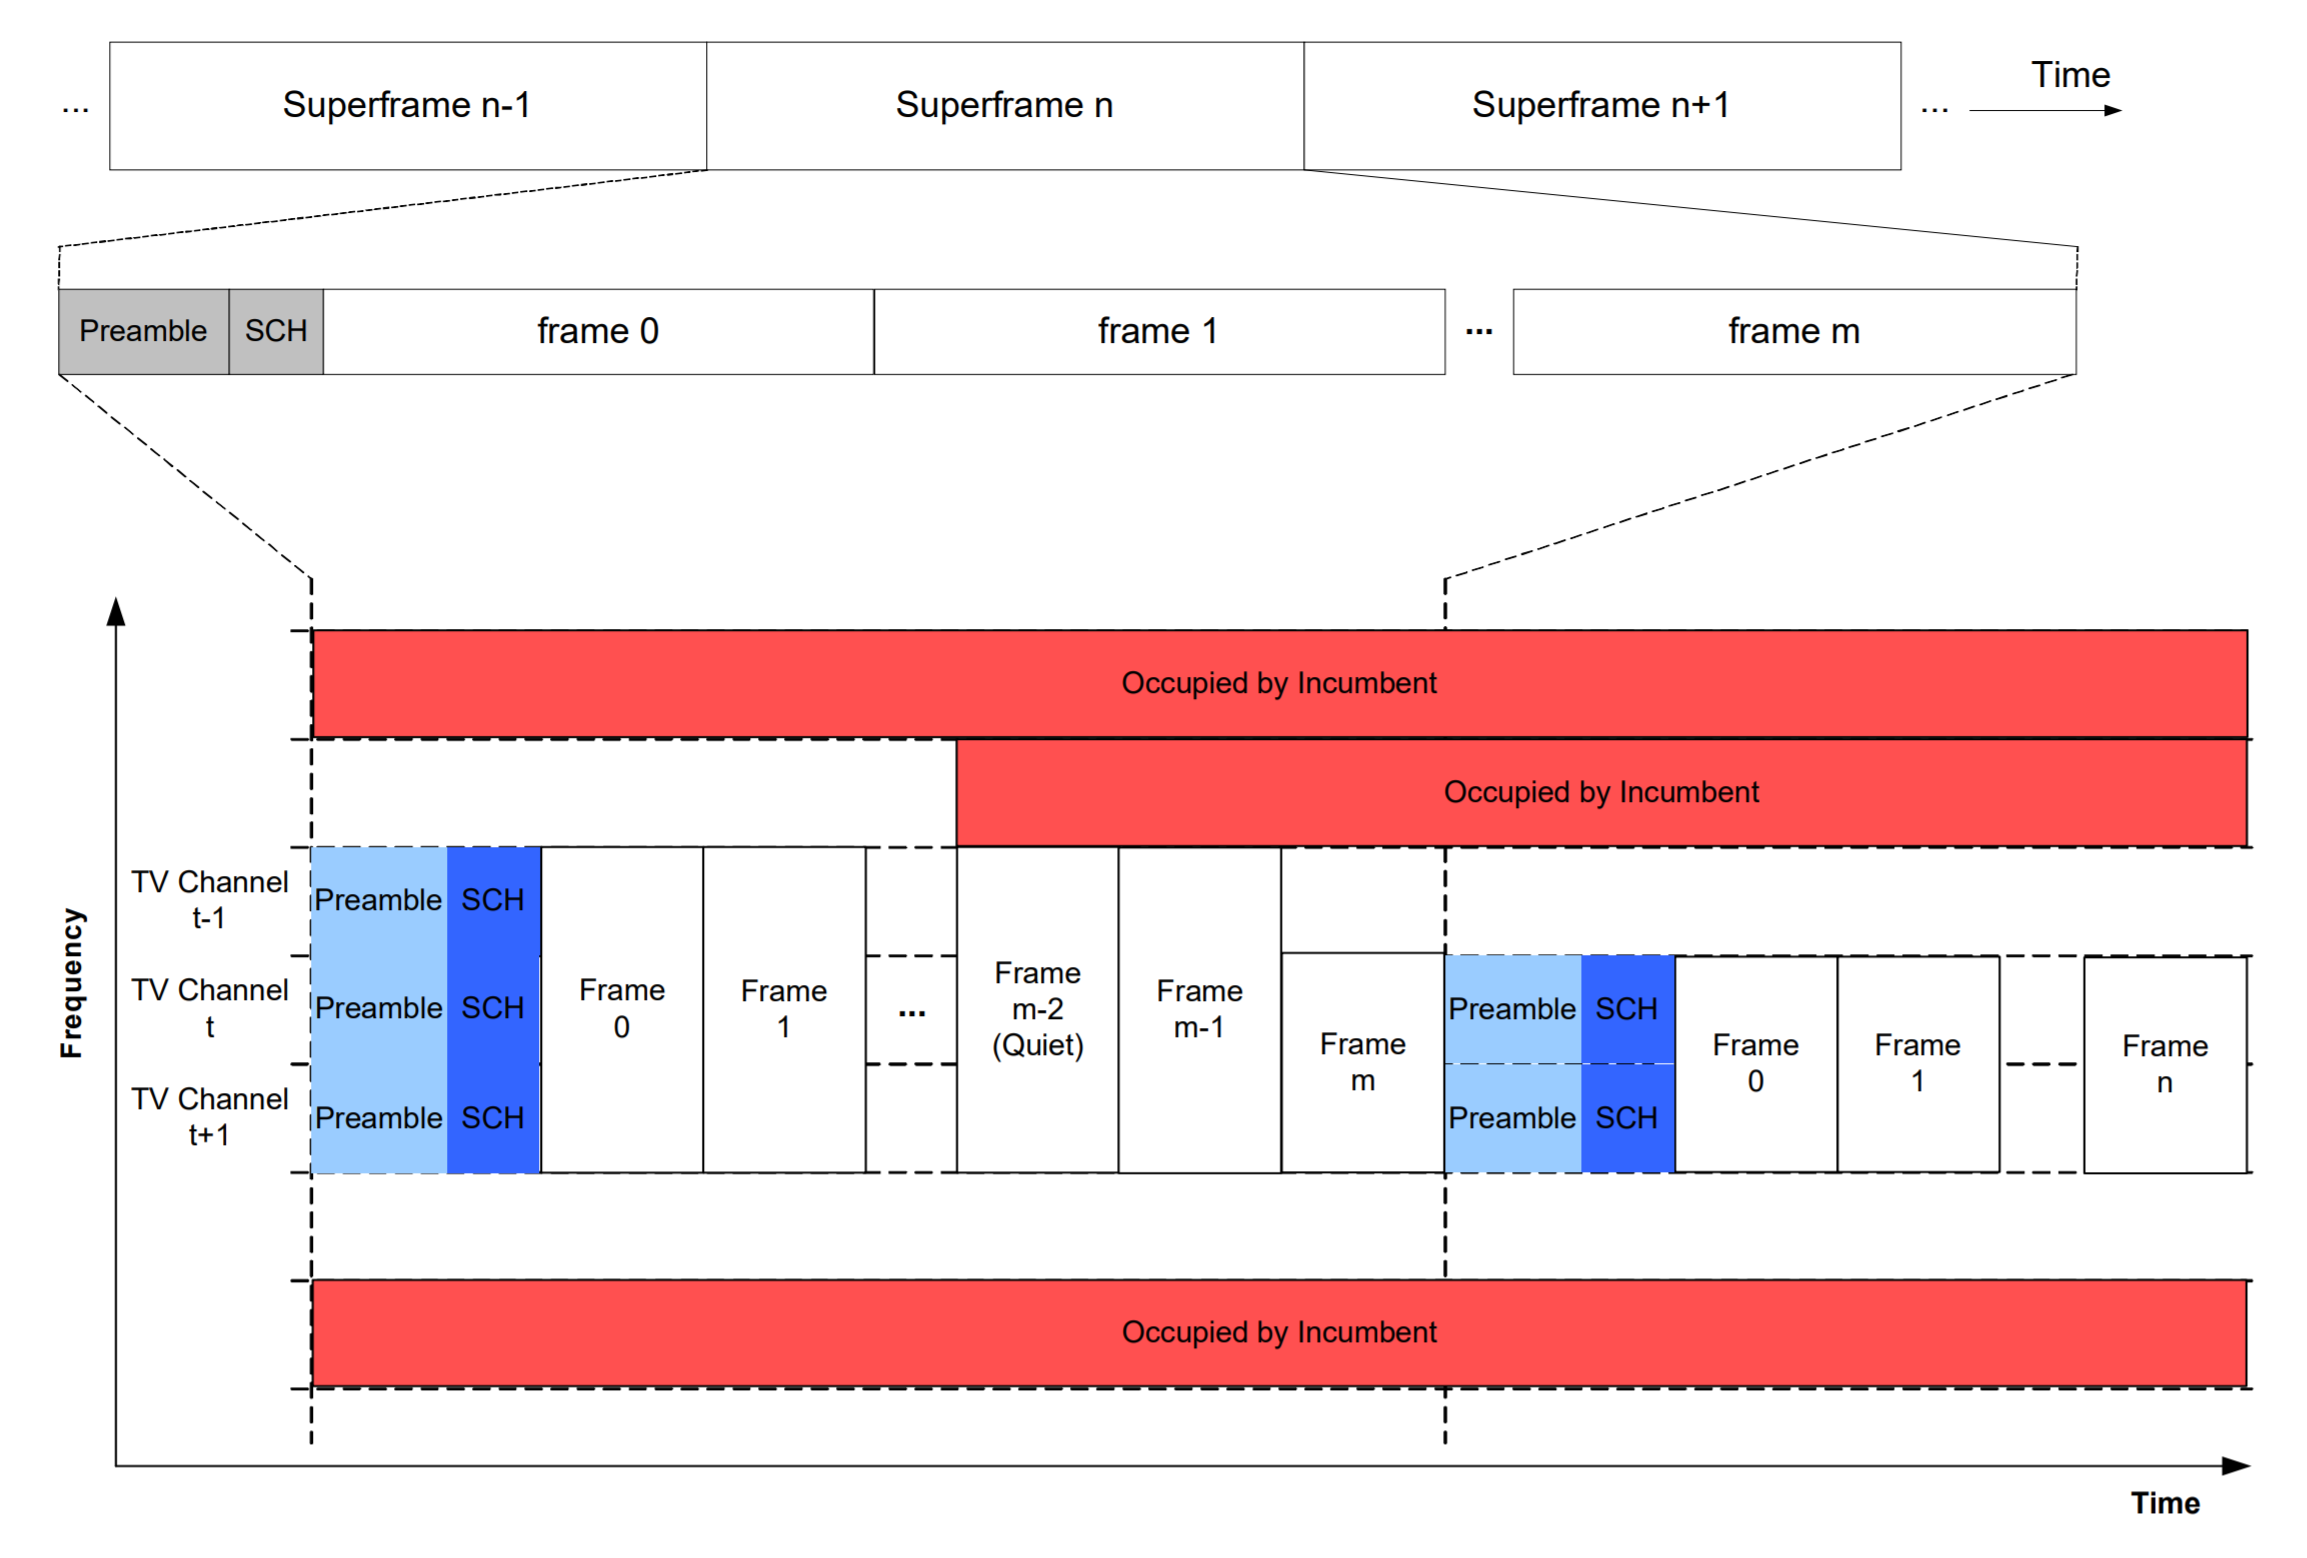
\includegraphics[width=12cm]{figures/frame.png}
\caption{Frame Structure \cite{ieee_802_22}}
\label{fig:frame}
\end{figure}

When implementing CR device, regulation suggests to take note of the following hardware characteristics:
\begin{itemize}
  \item Receiver sensor sensitivity 
  \item Channel sensing time
  \item Hit rate
  \item False alarm
\end{itemize}
Looking at the sensitivity of the device, a better sensor senses and reacts to the environment in much longer range and shorter 
time. Hit rate and false alarm of the hardware relate closely to the system integration design. You can find most of these statistical
value in the datasheet of the module parts.



\chapter{Software Design}
\section{Arduino Support}
Going into the software design scheme, some considerable useful library support would be those from the Arduino platform. 
Before software implementation, the main hardwares parts were chosen for this project. More detail on the parts choices
will be explained in the next chapter. 
Since the micro controller unit (MCU) and transceiver module are decided to be Arduino Nano with chip model ATMEGA328 and 
chip model CC1101, the three libraries of the testbed built out of are \texttt{<Arduino.h>}, \texttt{<EEPROM.h>} and \texttt{<ELECHOUSE\_CC1101.h>}. 
In the Arduino header file, there are lists of Digital, Analog and Advanced input/output (I/O) functions that are pre-built
for programmer uses \cite{arduino_reference}. It also declares standard scopes of the data types and the constants.
The Arduino library gives full access of the fundamental control structure, such as ``loop'', ``if'', ``return'' statements,
etc. Above categories are some of the handy functions that have been used in the CR testbed. Next, to keep track of the 
emulation result, each CR device will need to record some important occurrences during the experiment somewhere.
The built-in electrically erasable programmable read-only memory (EEPROM) in Arduino Nano is a great place to store data. \texttt{<EEPROM.h>} includes all the basic
functions that the project needs within the library. Lastly, the project utilizes
the \texttt{<ELECHOUSE\_CC1101>} files by developer, Michael, from Elechouse Company. It provides basic subroutines
for parameterizing the CC1101 transceiver chip as it communicates with the MCU. 
In Github, username, Little Satan, modified a much more user friendly version of the Library called, 
\texttt{SmartRC-CC1101-Driver-Lib}. It further develops sets of classes and functions, leaving users an easy setup
at a high level abstraction; that is, the transceiver library this project is using. Below are few lines of code in 
the programming scripts when referencing the tools.
\newline
\begin{lstlisting}[caption={Library used in the testbed},captionpos=b]
// Include Libraries
#include <Arduino.h>
#include <EEPROM.h>
#include <ELECHOUSE_CC1101_SRC_DRV.h>
\end{lstlisting}


The overall structure of the testbed is built using the Arduino library. To get access to all common constants value easier, 
it initializes the numbers in the header files. Arduino platform allows the building and use of custom library, which users can take advantage
of, making a much more suitable subroutine for specific operation. One other function that the testbed uses for device performance indication 
is the LED manipulation in the digital general purpose input output (GPIO) port. The way it records data is by storing to the build-in
EEPROM inside the ATMEGA328 chip. It monitors data through 
serial peripheral interface (SPI) communication between the CR device and the graphical user interface (GUI) within the client machine.
In \texttt{<ELECHOUSE\_CC1101\_SRC\_DRV.h>} and related compiled files, modified functions provide direct manipulation from MCU 
to CC1101 chip through SPI as well. The handy functions convert user level instructions to digital signals, which then also be transferred 
through SPI. With every data retrieval MCU can react based on sensed value. The summary of the functions used are included in
Table~\ref{tab:function}, Table~\ref{tab:function2} and Table~\ref{tab:function3}.

\section{Protocol Setup}

This testbed emulates operational and authentication methods that radios use in the air. During the experimental process, 
the Base Station (BS), Customer Premises Equipments (CPE) and Licensed Band Users (LBU) communicate and interfere using 
a set of specific protocols. They send messages through custom packets one after another to simulate frames. The testbed simplified 
the process by encoding four fields in a packet, the operational code, payload, source ID and destination ID, as Figure~\ref{fig:packet} describes. 
Each field is 8 bits or 1 byte long. The message packet in total is 4 bytes in length. The operational code is responsible for identifying the 
action that the device is taking, as well as the device type. In the payload section, it functions differently with a different operational code.
The source ID and the designation ID usually refers to the message packet itself. For the full set of message structures and their functions, 
please refer to Table~\ref{tab:structure}.


\begin{figure}[ht]
\centering
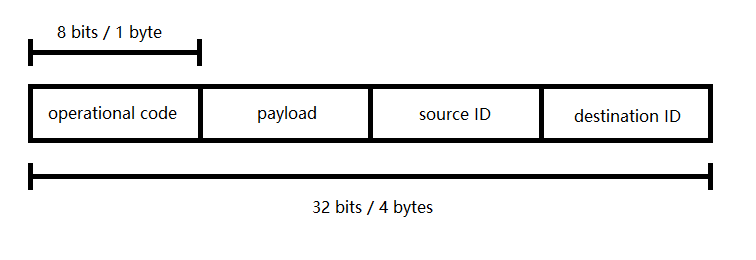
\includegraphics[width=12cm]{figures/packet.png}
\caption{Message Packet Structure}
\label{fig:packet}
\end{figure}

Some of the communication scenarios will be discussed below. When a CPE wants to setup a connection with another CPE, the device needs to 
identify its actions by putting a corresponding operational code, a number indicating desired connection duration, its own user ID number, and 
the target user ID number. It sends at the reserved channel and waits for a response back from BS, the centralized unit of the network, until the timer expires. 
\begin{figure}[ht]
  \subfloat[Perfect Connection Setup]{
	\begin{minipage}[c][1.5\width]{
	   0.4\textwidth}
	   \vspace{-14mm}
	   \centering
	   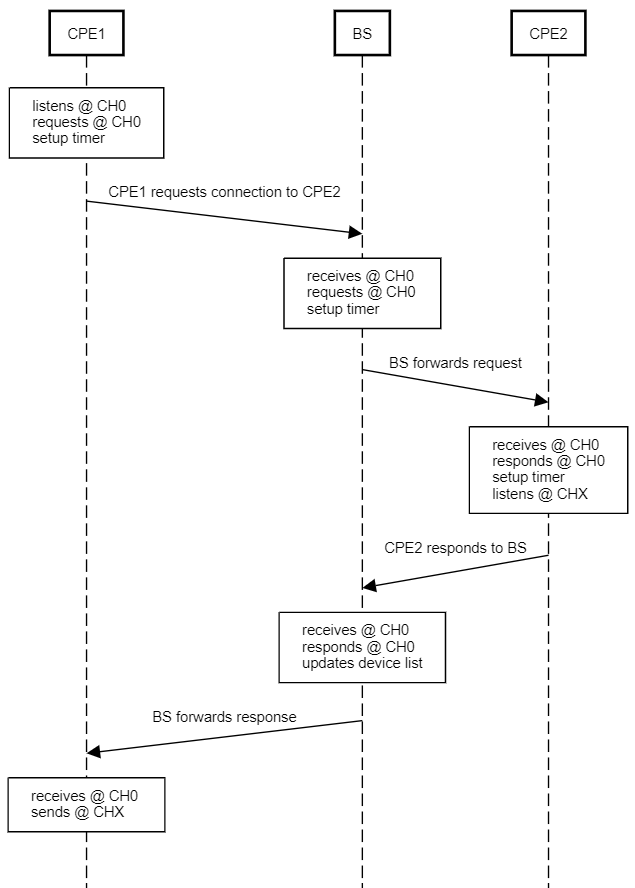
\includegraphics[width=0.8\textwidth]{figures/sequence_diagram_perfect_com.png}
	\end{minipage}}
 \hfill 	
  \subfloat[Message Dropped at the 1st Transmission]{
	\begin{minipage}[c][1.5\width]{
	   0.4\textwidth}
	   \centering
	   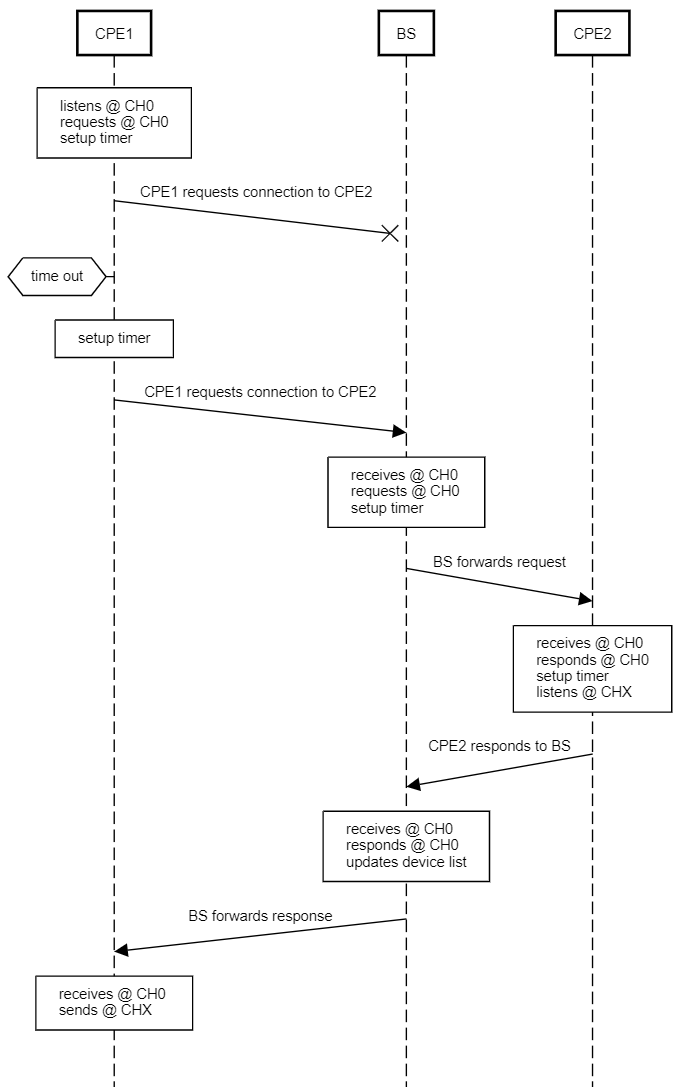
\includegraphics[width=0.85\textwidth]{figures/sequence_diagram_first_miss_com.png}
	\end{minipage}}
\caption{Connection Setup}
\label{fig:connection_setup}
\end{figure}


BS catches the messages and decodes them, which could be further processed by program logic. BS then forwards the message to the target
CPE by inserting an assigned channel to the payload field. After transmitting, BS sets up a timer and waits for a response. As the target
device receives a request from BS, it responds right back with a corresponding operational code and confirms the channels with the same payload
information as the incoming message. Note, that in this packet, the source ID will be the target CPE and the destination ID will be the 
original requesting CPE ID. BS catches the response; it forwards back to the requesting CPE to let it know that the connection has been set up
successfully. A perfect scenario is demonstrated by the sequence diagram in Figure~\ref{fig:connection_setup}(a). However, if the initial 
request could not reach to BS by the time the timer expires, the source CPE would send another request until it receives a desired response from
BS. Figure~\ref{fig:connection_setup}(b) shows a successful connection after the first transmission miss. If the connection process is interrupted or
any of the devices could not catch the response, like those sequence diagrams shown in Figure~\ref{fig:other_miss_cases}, the source CPE would have to try the whole process again when the timer expires.

\begin{figure}[ht]
  \subfloat[Message dropped at the 2nd]{
	\begin{minipage}[c][1.4\width]{
	   0.31\textwidth}
	   \vspace{-20.5mm}
	   \centering
	   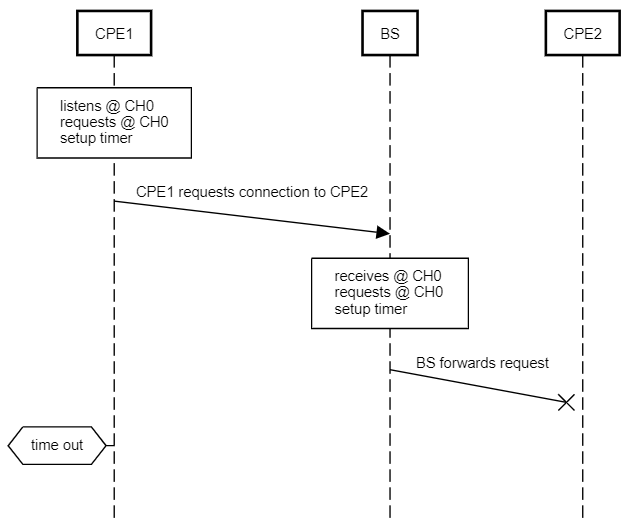
\includegraphics[width=1\textwidth]{figures/sequence_diagram_second_miss.png}
	\end{minipage}}
 \hfill 	
  \subfloat[Message dropped at the 3rd]{
	\begin{minipage}[c][1.4\width]{
	   0.31\textwidth}
	   \vspace{-13mm}
	   \centering
	   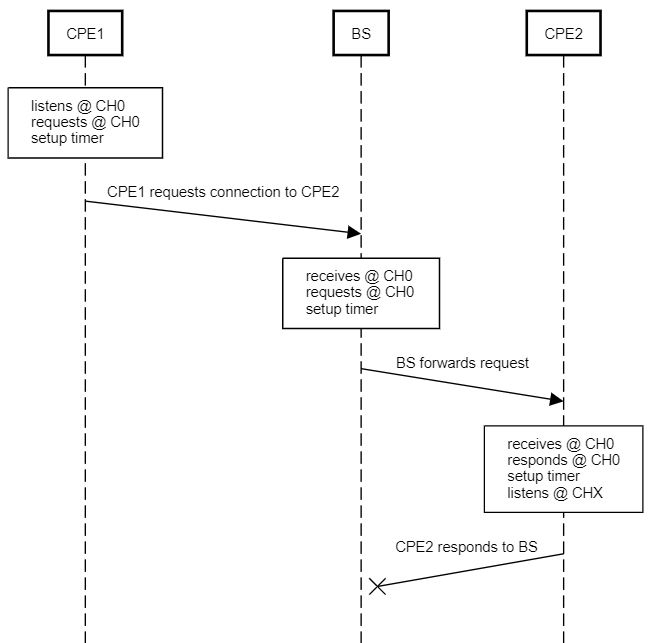
\includegraphics[width=1\textwidth]{figures/sequence_diagram_third_miss.png}
	\end{minipage}}
 \hfill	
  \subfloat[Message dropped at the 4th]{
	\begin{minipage}[c][1.4\width]{
	   0.31\textwidth}
	   \vspace{0mm}
	   \centering
	   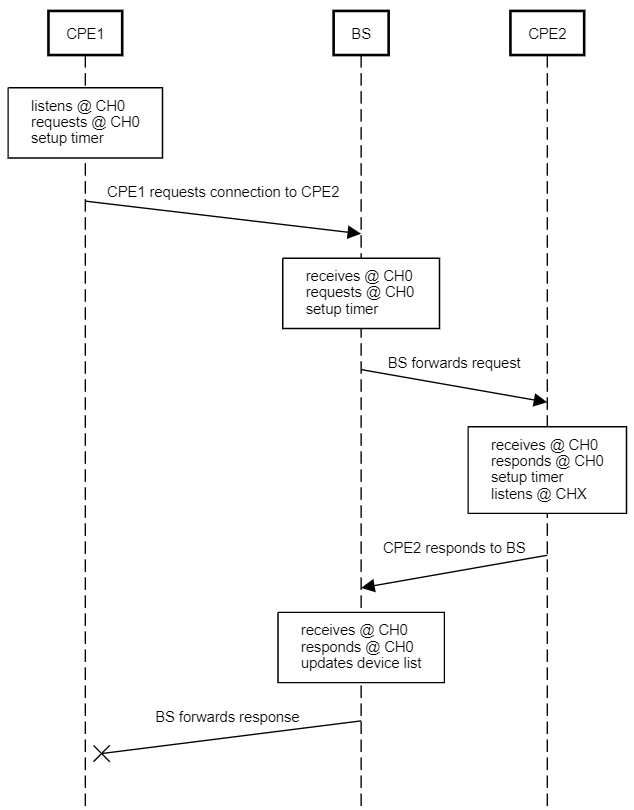
\includegraphics[width=1\textwidth]{figures/sequence_diagram_fourth_miss.png}
	\end{minipage}}
\caption{Other Miss Cases}
\label{fig:other_miss_cases}
\end{figure}

Upon establishing a connection, two CPEs would send and receive data at a designated channel that is different from the reserved channel. A successful data transfer results in both CPEs returning to the reserved channel normally shown in Figure~\ref{fig:with_lbu}(a). During the data transfer period, if any LBU happens to transmit at the frequency that CPEs are at, both CPEs are forced to drop the in progress communication at the current channel, like the one in Figure~\ref{fig:with_lbu}(b). A new channel connection is required to be set up. 



\begin{figure}[ht]
  \subfloat[Successful Data Transfer]{
	\begin{minipage}[c][1.7\width]{
	   0.4\textwidth}
	   \centering
	   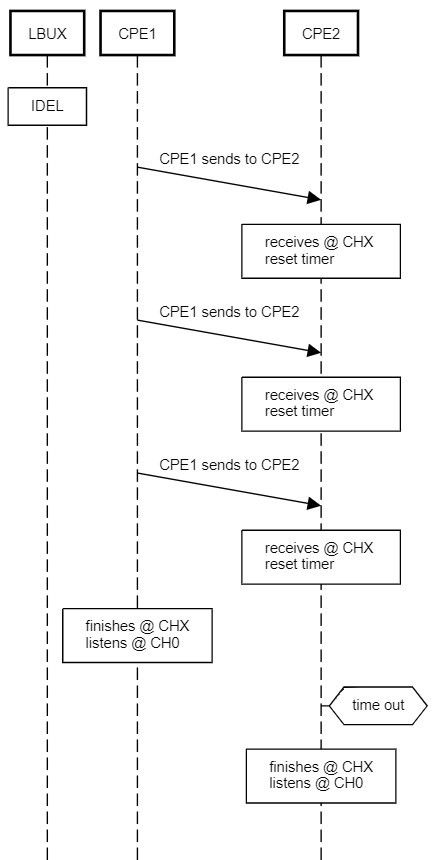
\includegraphics[width=0.8\textwidth]{figures/sequence_diagram_no_interrupt.png}
	\end{minipage}}
 \hfill 	
  \subfloat[Data Transfer Interruption]{
	\begin{minipage}[c][1.7\width]{
	   0.4\textwidth}
	   \vspace{-33mm}
	   \centering
	   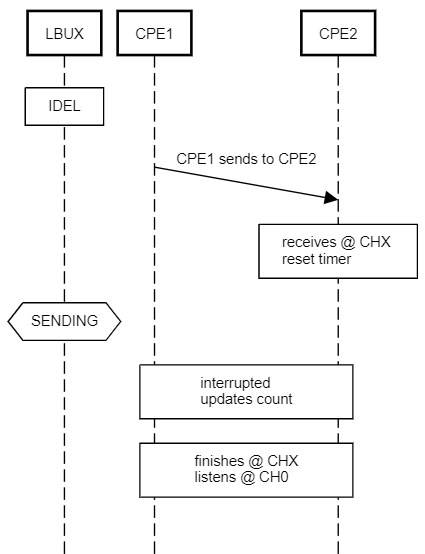
\includegraphics[width=0.8\textwidth]{figures/sequence_diagram_interrupt.png}
	\end{minipage}}
\caption{With Licensed Band Users}
\label{fig:with_lbu}
\end{figure}

\section{Establish Library}

The benefits of establishing specific libraries are making both the repetitive, complex logic easier to use and the process more scalable. 
Each library comprises of two files, a header file with all the defined functions and a C++ file that codes in all the logics. Some constants are 
also defined in the header file. These libraries generally help project development in the long run. 
Next, are the two customized libraries, \texttt{RADIO} and \texttt{TEST}, that were made and included in this testbed. For the full description of operational code constants in the header files, please refer to Table~\ref{tab:structure}.

\subsection{RADIO}
\texttt{RADIO} library integrates those necessary subroutines to manipulate the transceiver module into short accessible function calls. Notice that the project avoids channel interference by defining a large channel separation. \texttt{switchChannel(byte)} subroutine makes sure it switches to the correct frequency. To understand and use all functions in this library, follow the method descriptions and formats that are listed below.

\begin{itemize}
  \item \texttt{void initialize\_trans(void)}\newline
  Description: it sets up initial parameters for the CC1101 registers, using some of the \texttt{ELECHOUSE\_CC1101\_SRC\_DRV} functions, including transmission mode, transmission modulation, base frequency, receiver bandwidth, etc.\newline
  Format: input NONE; output NONE.
  \item \texttt{void receiveMessage(int, byte *, byte, byte)}\newline
  Description: it utilizes \texttt{CheckRxFifo()} and \texttt{CheckCRC()} from \texttt{ELECHOUSE\_CC1101}. Based on user defined device type and target ID, when the corresponding flag is raised, it retrieves the data in the air and decodes the message, and then puts it back to the message placeholder at the end.\newline
  Format: input receive maximum duration, received message placeholder, device type and target ID; output NONE.
  \item \texttt{void sendMessage(int, byte *)}\newline
  Description: it encodes the message in the input placeholder and sends it to the air throughout the duration time period.\newline
  Format: input transmit duration and transmit message placeholder; output NONE.
  \item \texttt{void switchChannel(byte)}\newline
  Description: it switches channels by modifying CC1101 registers based on the defined channel separation.\newline
  Format: input channel number; output NONE.
  \item \texttt{void encode(byte *, byte *)}\newline
  Description: it merges packet fields into a condensed buffer for transmission in the air.\newline
  Format: input packet message separated in fields; output condensed packet data.
  \item \texttt{void decode(byte *, byte *)}\newline
  Description: it decodes the condensed data stream into logical processable packet fields. \newline
  Format: input packet raw data buffer; output packet message separated in fields.
\end{itemize}




\subsection{TEST}
\texttt{TEST} library is made for generalizing most of the CR testing environment setup. In the header file, the user should put all of the test cases and stimulus. The constants defined at the top of the file apply to the current experiment, such as the schedule size, emulation duration, algorithm type, number of devices under test (DUT), etc. There are also handy subroutines developed for recording and monitoring the data. To understand and use all functions in this library, follow the method descriptions and formats that are listed below.

\begin{itemize}
  \item \texttt{void initialize\_scheduleList(byte, byte *)}\newline
  Description: it places the schedule in the LBU programs for them to follow accordingly.\newline
  Format: input LBU ID and schedule array placeholder; output NONE.
  \item \texttt{void record(int, byte, byte)}\newline
  Description: it first stores time and then data to the given memory location.
  Format: input memory location, time data and value data; output NONE.
  \item \texttt{void report(void)}\newline
  Description: it displays all data from the memory to the monitor in the client machine.\newline
  Format: input NONE; output NONE.
\end{itemize}

\section{Program Module}

This section goes into the software flow of each individual type of device. During physical testing, BS, CEPs and LBUs first establish a regional network shown in Figure~\ref{fig:network}. For this testbed, all devices communicate through broadcasting, especially the BS. CPEs are software defined as enabling point to point, which means two CPEs can talk to each other without the BS in the middle after the channel is established. The LBUs interrupt also in a broadcasting way. The primary and the secondary devices interact with each other based on the testing stimulus or the assigned tasks. Some outcomes of the interaction would be recorded individually by the CPEs. To explain their operating relationship and the flow of the program, it includes state-diagram-level abstractions on how they run in the experiment. The complete code of the project is included in this link: \newline \url{https://github.com/SaltFishBoi/cognitive_radio_network_environment_deployment} 

\begin{figure}[ht]
\centering
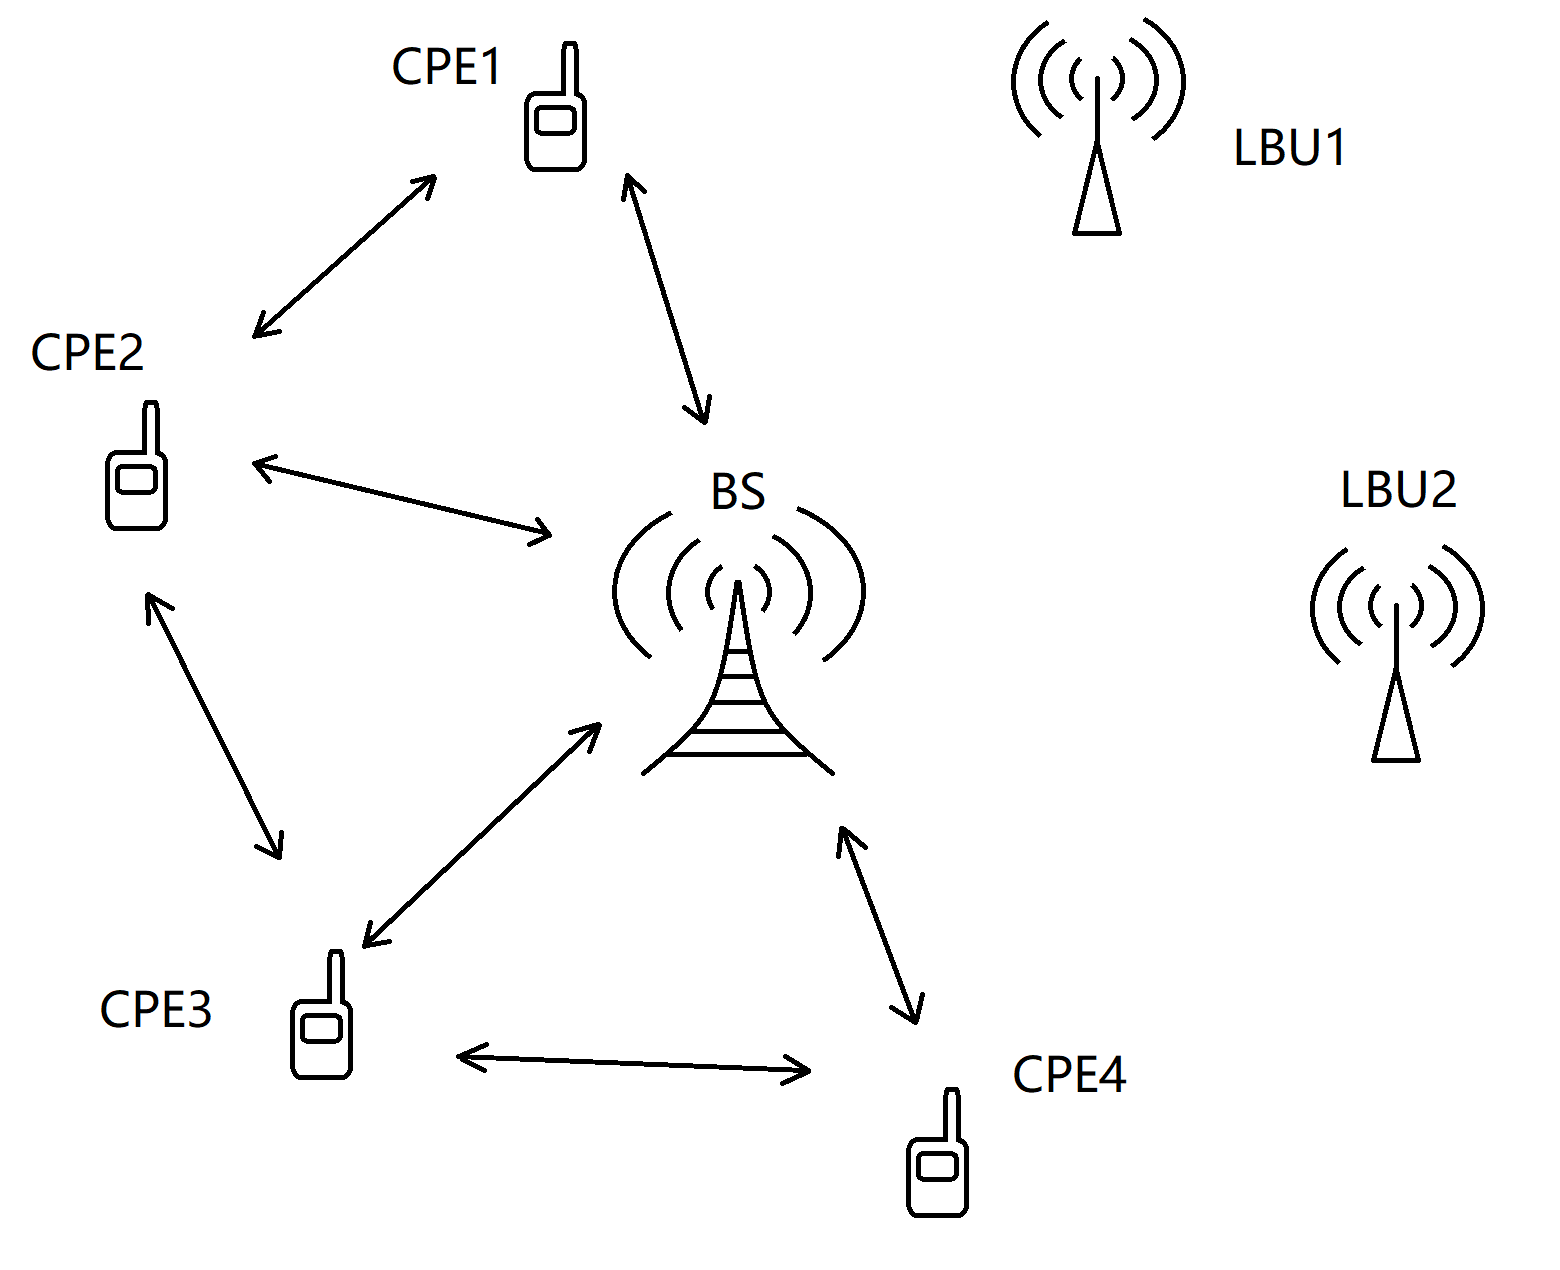
\includegraphics[width=12cm]{figures/network.png}
\caption{Cognitive Radio Regional Network}
\label{fig:network}
\end{figure}


\subsection{Base Station}

The centralized unit for CRN is BS. It is responsible for sensing the environment and overseeing the spectrum assignment. The station starts by setting all necessary indicators and register values for the transceiver module. Next it initializes all the tables, a mechanism that keeps track of the changing environment. The tables include the spectrum table, client table, and the selection table for more advanced algorithms. The experiment requires every device under the test to be synchronized in time. Being the central unit of the network, the BS needs to synchronize the time with the rest of the devices in the next step. After that, the program performs the main process, which can be described by the state diagram shown in Figure~\ref{fig:state_diagram_bs}. The BS is running in two states, listening to any incoming request and responding to a request. During the listening state, it relies on the functions in \texttt{RADIO} library to retrieve messages sent from CPEs in the air. Once it receives a valid request from a CPE, it goes to responding state, based on the algorithm specified in the test. It selects the corresponding channel and sends that request to the target CPE. It then waits for a response back from the same CPE with the target ID. If it never catches the response from the target CPE, it will go back to the listening state as if the message had been dropped. If it catches a response from the target CPE, it would update the client list status because two CPEs would be talking soon. Upon sending a response back to the source CPE, the BS has created a successful connection and will go back to the listening state. Based on the algorithm requirement, the BS senses the environment and updates the selection table periodically.

\begin{figure}[ht]
\centering
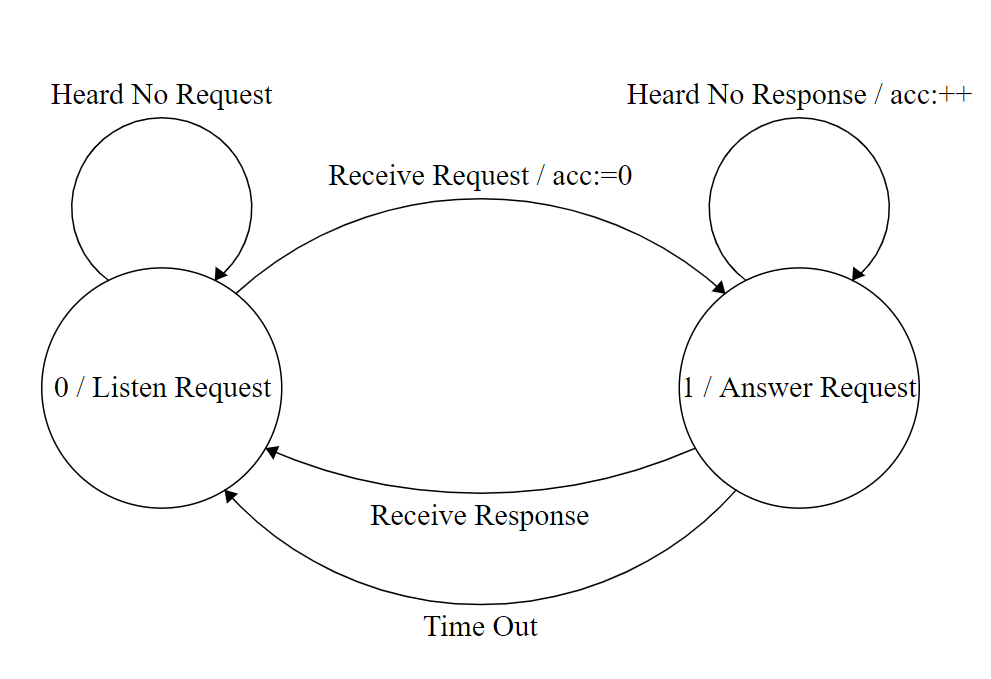
\includegraphics[width=12cm]{figures/state_diagram_bs.png}
\caption{State Diagram Base Station}
\label{fig:state_diagram_bs}
\end{figure}


\subsection{Customer Premises Equipment}
All secondary devices, CPEs, need to first set the indications and register values for the transceiver modules as well. Next in the CPE program, it synchronizes with the BS. After that, in the CPE main process loop, it runs at one of three states as shown in Figure~\ref{fig:state_diagram_cpe}. All CPEs initially try requesting BS for a connection to another CPE. If the BS picks up the message and responds back with an assigned channel before the request timer expires, the source CPE would hop into the assigned channel and begin sending data. Then CPE sender would be done sending if it goes through the whole scheduled duration without interruption. The sender is capable of sensing if the channel is busy, in which LBU occupies the channel. It returns back to the request state if any of the two cases occurs. The occurrences would be accumulated and stored in the memory.

\begin{figure}[ht]
\centering
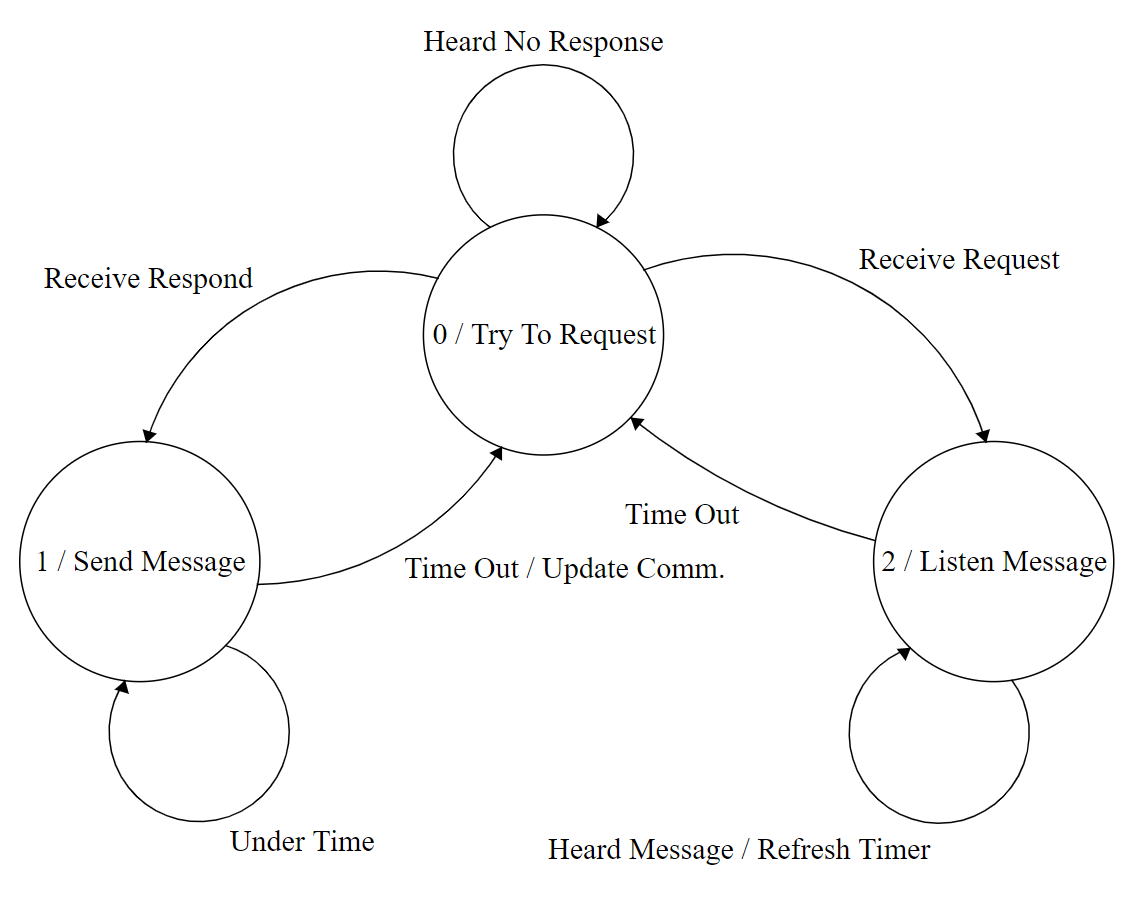
\includegraphics[width=14cm]{figures/state_diagram_cpe.png}
\caption{State Diagram Customer Premise Equipment}
\label{fig:state_diagram_cpe}
\end{figure}

If CPE hears nothing back from BS that is associated with its ID throughout the request time period, CPE will send the request again after a constant time of delay. During the requesting process, if CPE hears a connection request from another CPE forwarded by BS, it would confirm the channel and respond back to BS. In this case, it will hop into the assigned channel and go into the listening state. In that channel, it sets and refreshes a listening timer everytime it hears back from the CPE sender. It will go back to the request state when the timer expires or the channel is busy. 

The CPE finishes the process by taking the user defined experiment time into account. It emulates the real time, days and weeks in a much shorter period. By the end day that is set for the experiment, the CPE main process exits and the test is finished.  

\subsection{Licensed Band User}

LBU devices act as spectrum interrupters in this testbed. Again, LBUs need to first synchronize with all the rest of the device. After that, it initializes schedules with the \texttt{TEST} library. Based on the schedule and current synchronized time, LBU sends data at the designated channels. It loops the process until the experiment is done.


\begin{figure}[ht]
\centering
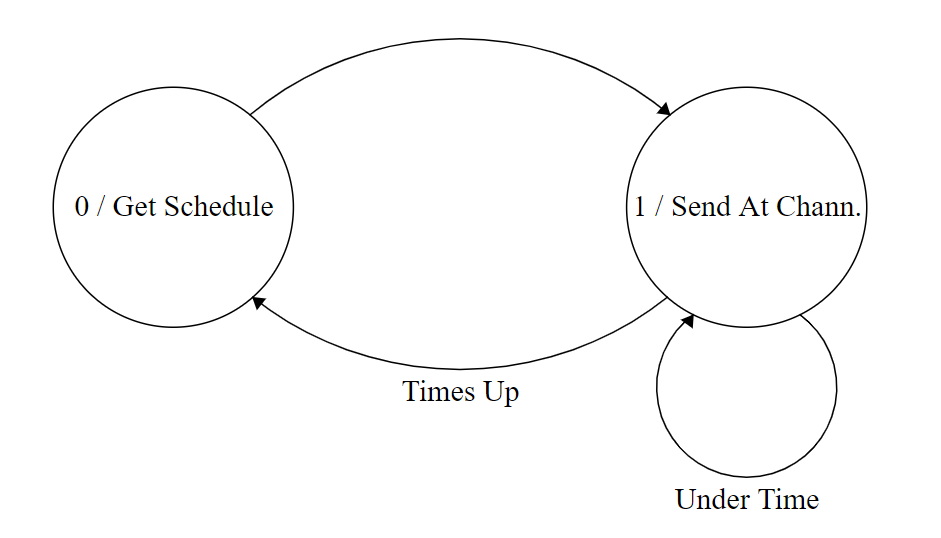
\includegraphics[width=12cm]{figures/state_diagram_lbu.png}
\caption{State Diagram Licensed Band User}
\label{fig:state_diagram_lbu}
\end{figure}

\chapter{Hardware Implementation}
\section{Modules Selection}

The previous chapter explains the libraries used in this testbed and discloses some of the components that construct the testing environment. This chapter points out the significance of picking certain hardwares and modules other than the software support. Mainly, when considering parts for the testbed, the project focuses on the hardware capability and cost. 

In terms of functionality, a CR device must be able to sense the environment and react to the current situation. Since it needs to sense the spectrum in the air, it requires some sort of receiver with an antenna. To be able to also send data in the air, it requires a transmitter. CC1101 module composes a CC1101 transceiver chip, a SubMiniature version A (SMA) antenna, and circuitry that wires between the chip and the interface. A 3D model of the hardware module is shown in Figure~\ref{fig:cc1101_module}, which was found in an associated component sale page.

\begin{figure}[ht]
\centering
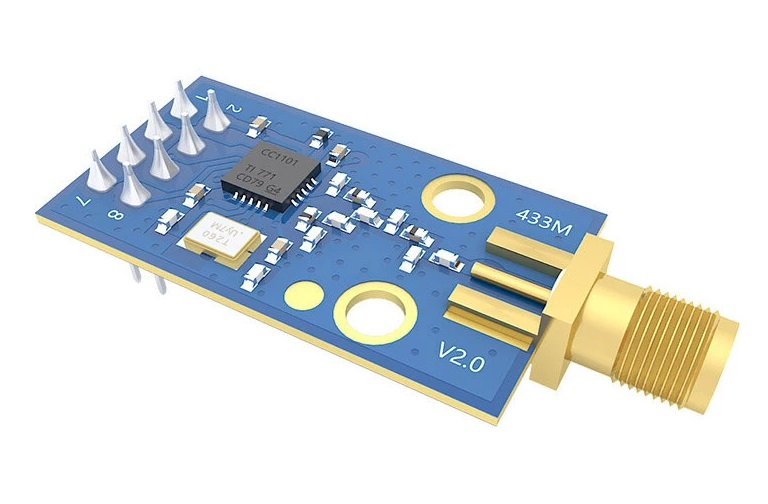
\includegraphics[width=12cm]{figures/cc1101_module.jpg}
\caption{CC1101 Transceiver Module \cite{cc1101_module}}
\label{fig:cc1101_module}
\end{figure}

The hardware characteristics of the CC1101 module are qualified in the following areas. All input required a voltage level below 3.6 V \cite{cc1101_module}. The operating current is well under 30 mA. If the typical operating I/O voltage is 3.3 V, the peak power is under 100 mW, which is acceptable for a testbed usage. It can transmit at a frequency range of 387 - 464 Mhz; the range falls in VHF range, which will fulfill the purpose of this project. The operation range of the transceiver can reach about 520 meters. It is capable of communicating with MCU through SPI. The operating temperature is designed for room temperature; it is specified to be between 40 - 85 \textdegree{}C.

The CC1101 module would only produce the environmental data that the CR device needs. There should be another module that processes the generated digital data from the transceiver. There are many hardwares that can process digital data, such as the single-chip microcontroller, field-programmable gate array (FPGA), digital signal processor (DSP), etc. Above all these, a well developed module board comes to mind; the Arduino Nano is the best candidate for this project due to its strong hardware support and flexible compatibility. The 3D model of this module is shown in Figure~\ref{fig:arduino_nano}, by artist Prashan Subasinghe.


\begin{figure}[ht]
\centering
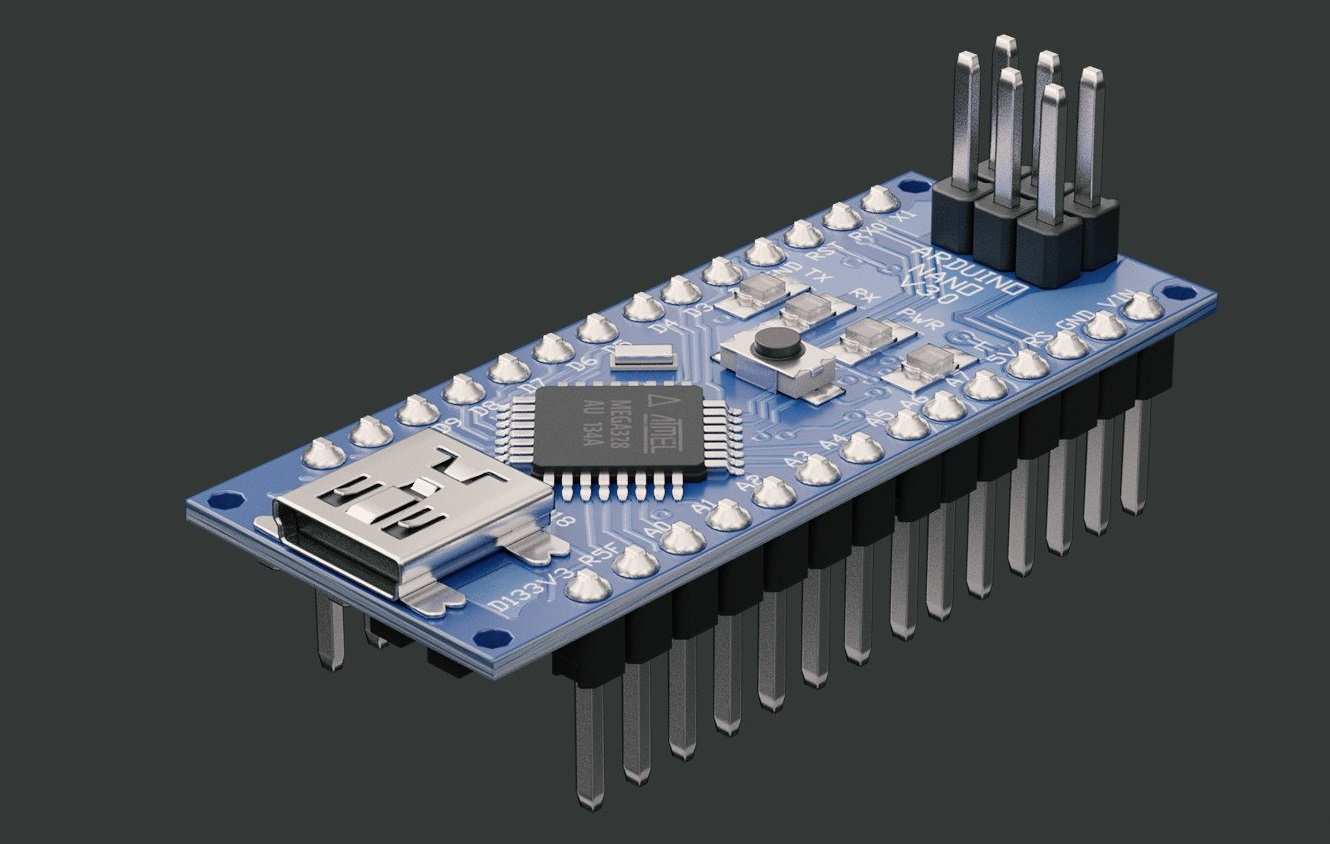
\includegraphics[width=12cm]{figures/arduino_nano.jpg}
\caption{Arduino Nano Module \cite{arduino_nano}}
\label{fig:arduino_nano}
\end{figure}

Arduino Nano uses the ATMEGA328 chip for the core of the part. Inside ATMEGA328 there is a micro process unit that can run at various clock speeds by dividing the default clock, 16 Mhz. In addition, ATMEGA328 has a built-in EEPROM with 1 kB capacity for data storage. That fulfills the project's data recording needs. Since it is used to drive the rest of the peripherals, it needs to produce a powerful I/O driven current. The data sheet shows it is capable of providing 40 mA per I/O pins. A 5 V operating voltage is perfect for the level shifters that have been selected for the project. The input voltage has a range from 7 - 12 V; this provides ranges of voltage-level for a 9 V running battery. There are plenty of digital I/O pins for all the traveling signals across the components. Its tiny size and power hardware make it stand out from the rest of MCU.


Furthermore, the testbed needs a control for starting the test. It is as simple as adding a switch that connects to the power. Lastly, during the experiment, the user should find it beneficial to have some kinds of indication of the device's performance or status. By flashing the LEDs at certain stages of the experiment process, the user can estimate the testing progress on the run. Figure~\ref{fig:block_diagram} shows the full top-level diagram. Note that in the final design, there are two sets of level-shifters between MCU and the transceiver module because the Arduino Nano produces and receives 5 V I/O, whereas CC1101 generates and takes in 3.3 V I/O. The components are generally easier to get with low prices. For the more complete specification of the hardware modules, please refer to Table~\ref{tab:arduino_spec} and Table~\ref{tab:cc1101_spec} in the Appendix. 

\begin{figure}[ht]
\centering
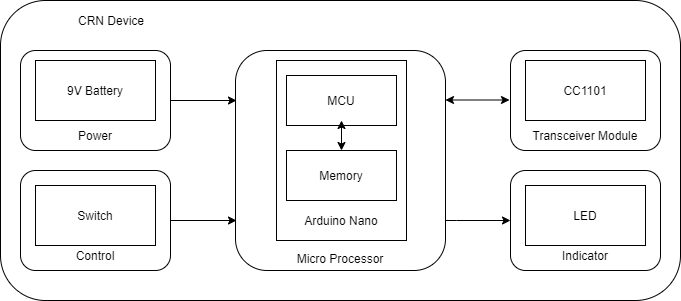
\includegraphics[width=12cm]{figures/new_block_diagram.png}
\caption{Top Level Block Diagram}
\label{fig:block_diagram}
\end{figure}


\section{Prototype Board}

The CRN testbed includes three different types of devices, BS, CPEs and LBUs. However, for the board development, all three types of devices are actually made by the same hardware layout. By uploading unique software programs, described from the previous chapter, to the device, they then behave differently. Figure~\ref{fig:prototype_board} is the complete prototype board schematic of the device. The figure is a back panel of the device with the exact wire routing to each node.


\begin{figure}[ht]
\centering
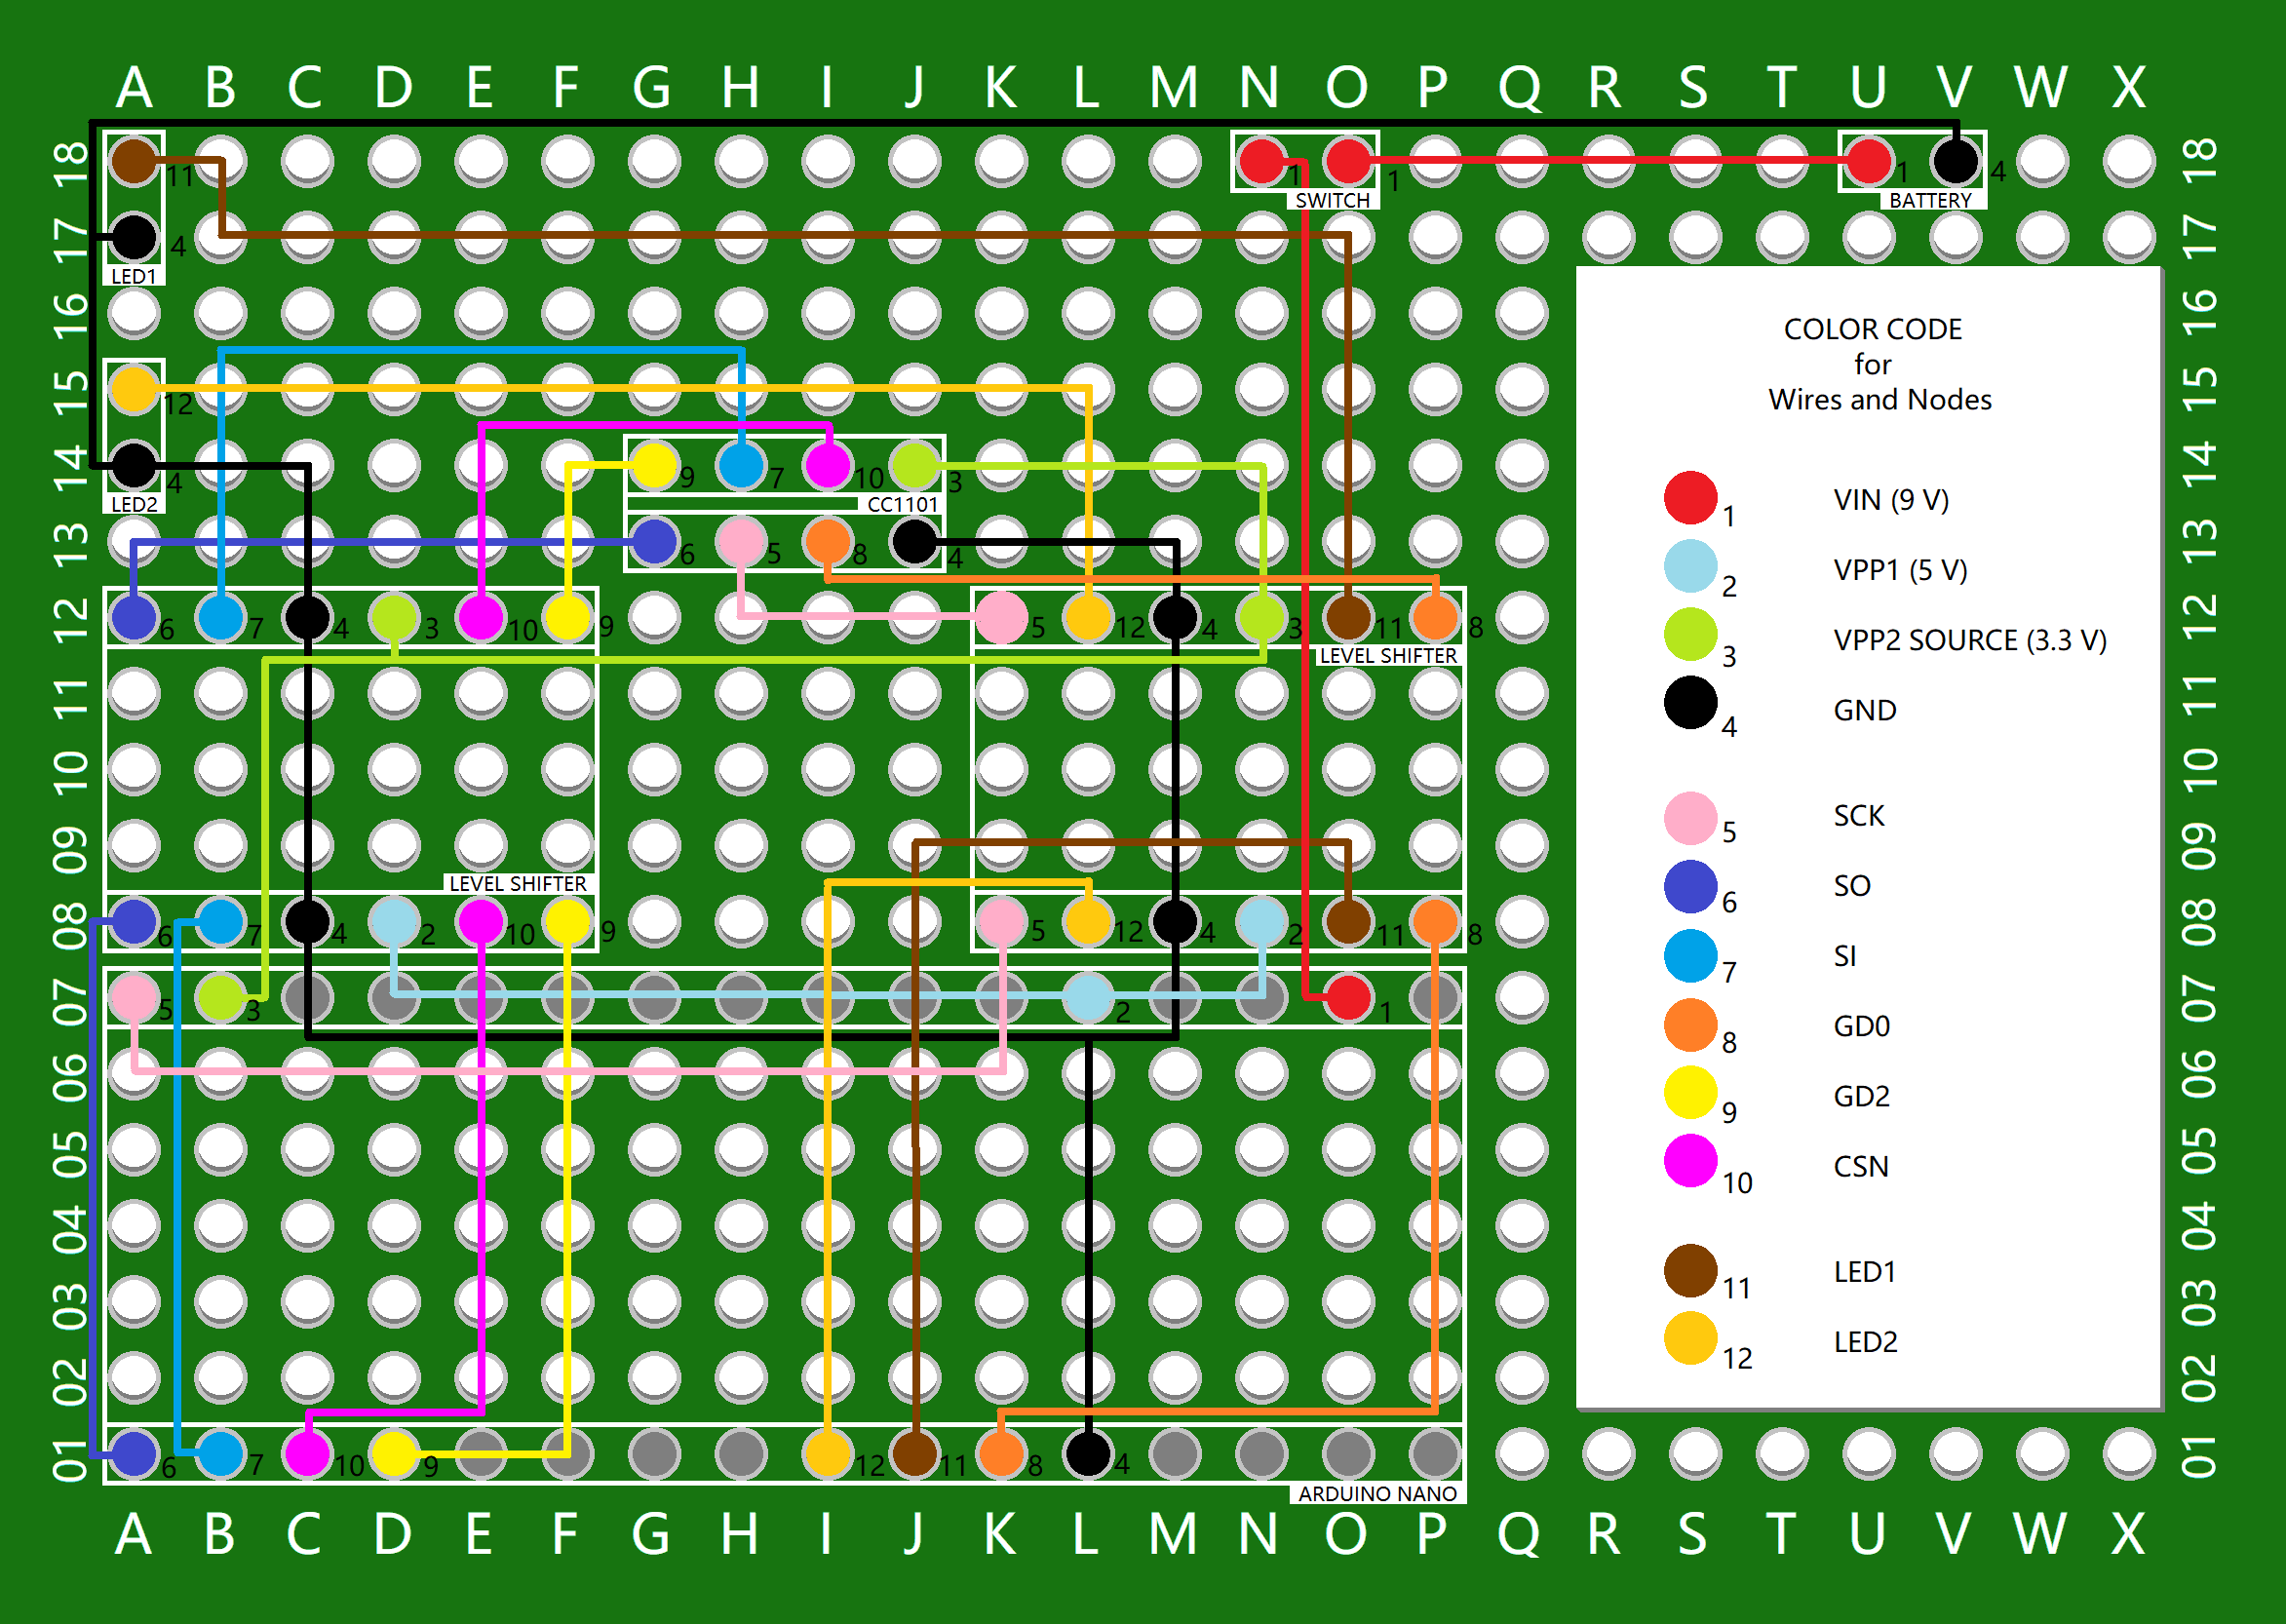
\includegraphics[width=14cm]{figures/clean_prototype_board.png}
\caption{Prototype Board Pin out and Wire}
\label{fig:prototype_board}
\end{figure}

After optimizing the placement and the wiring, components can fit on a 5 by 7 centimeter prototype board. On the side, there are reserved spaces for the power, and just enough space for a 9 V battery. The power switch, located at the top center of the board, is connected to the Arduino Nano power input and the power connector of the battery. The two LED indicators are located on the far top corner. One is blue; the other one is yellow. Toward the middle are a pair of soldered headers for the transceiver module. The two signal level-shifters are placed in the center of the layout. Each level shifter module is capable of shifting four I/Os. Two level-shifters are enough for all necessary signals in this project. On the bottom is the Arduino Nano. The power drives the Arduino machine; the Aruidno drives all the rest of the peripherals. Each color coded line represents the same wire connecting the pins and the headers. The legend on the side shows the color and number of the node and its corresponding pin name. With the detailed layout, the components are assembled into hand soldered devices, referring to Figure~\ref{fig:prototype_front_back_view}(a) and Figure~\ref{fig:prototype_front_back_view}(b) for the front and back view of the prototype.

\begin{figure}[ht]
    \centering
    \subfloat[\centering Prototype Front View]{{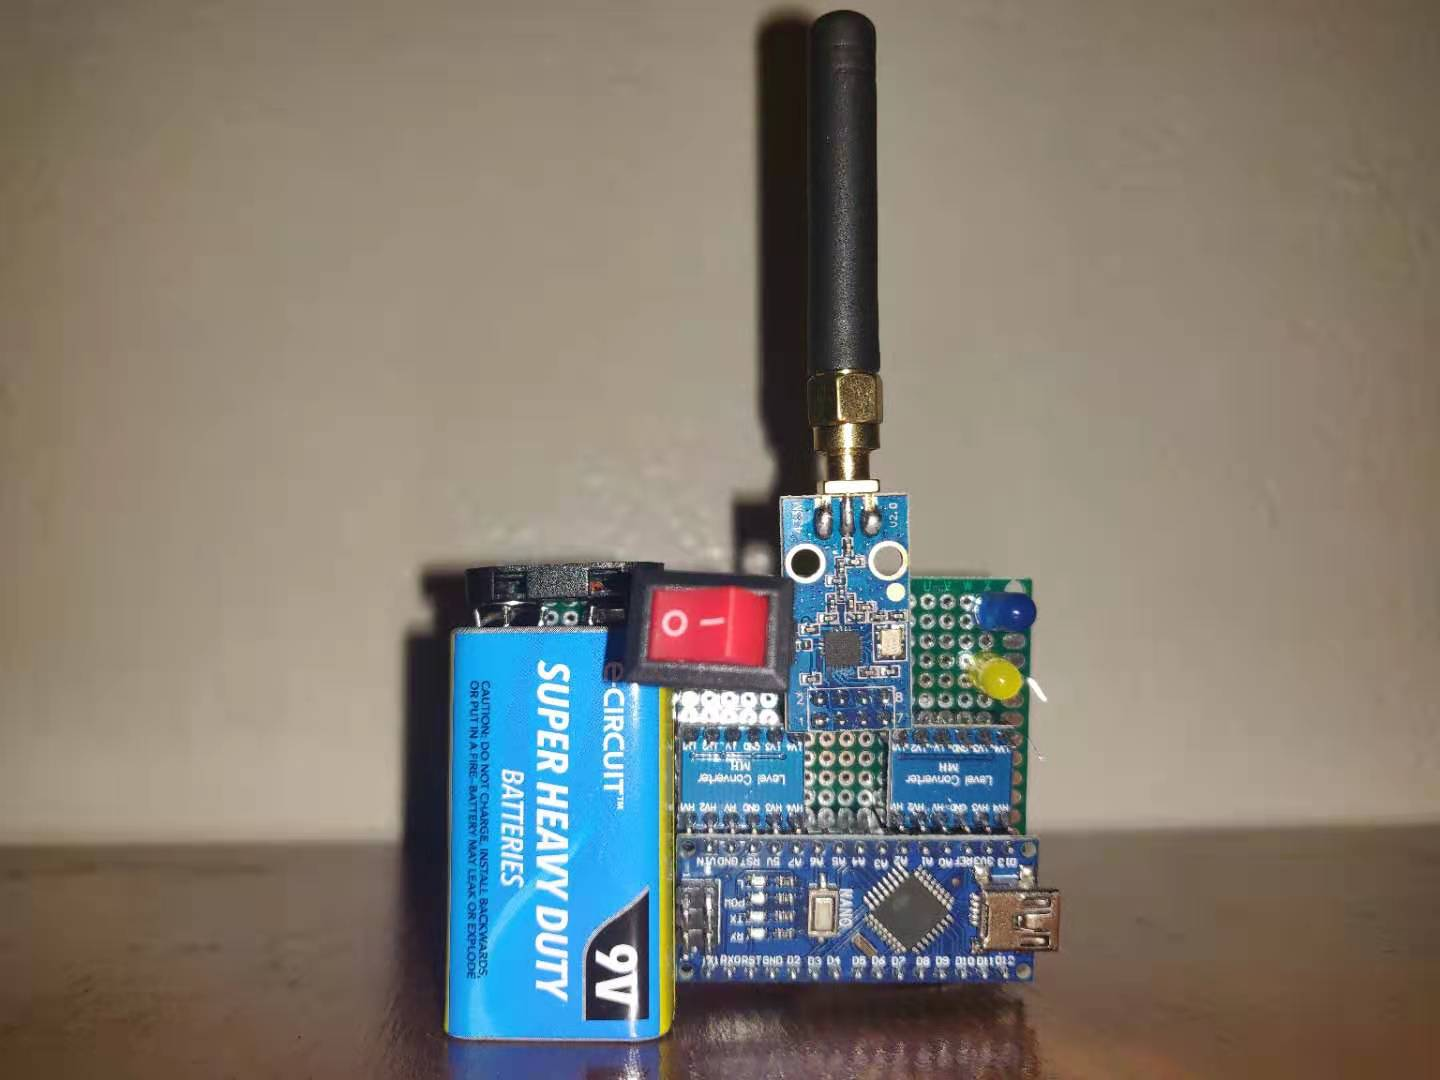
\includegraphics[width=6cm]{figures/prototype_front.jpg} }}%
    \qquad
    \subfloat[\centering Prototype Back View]{{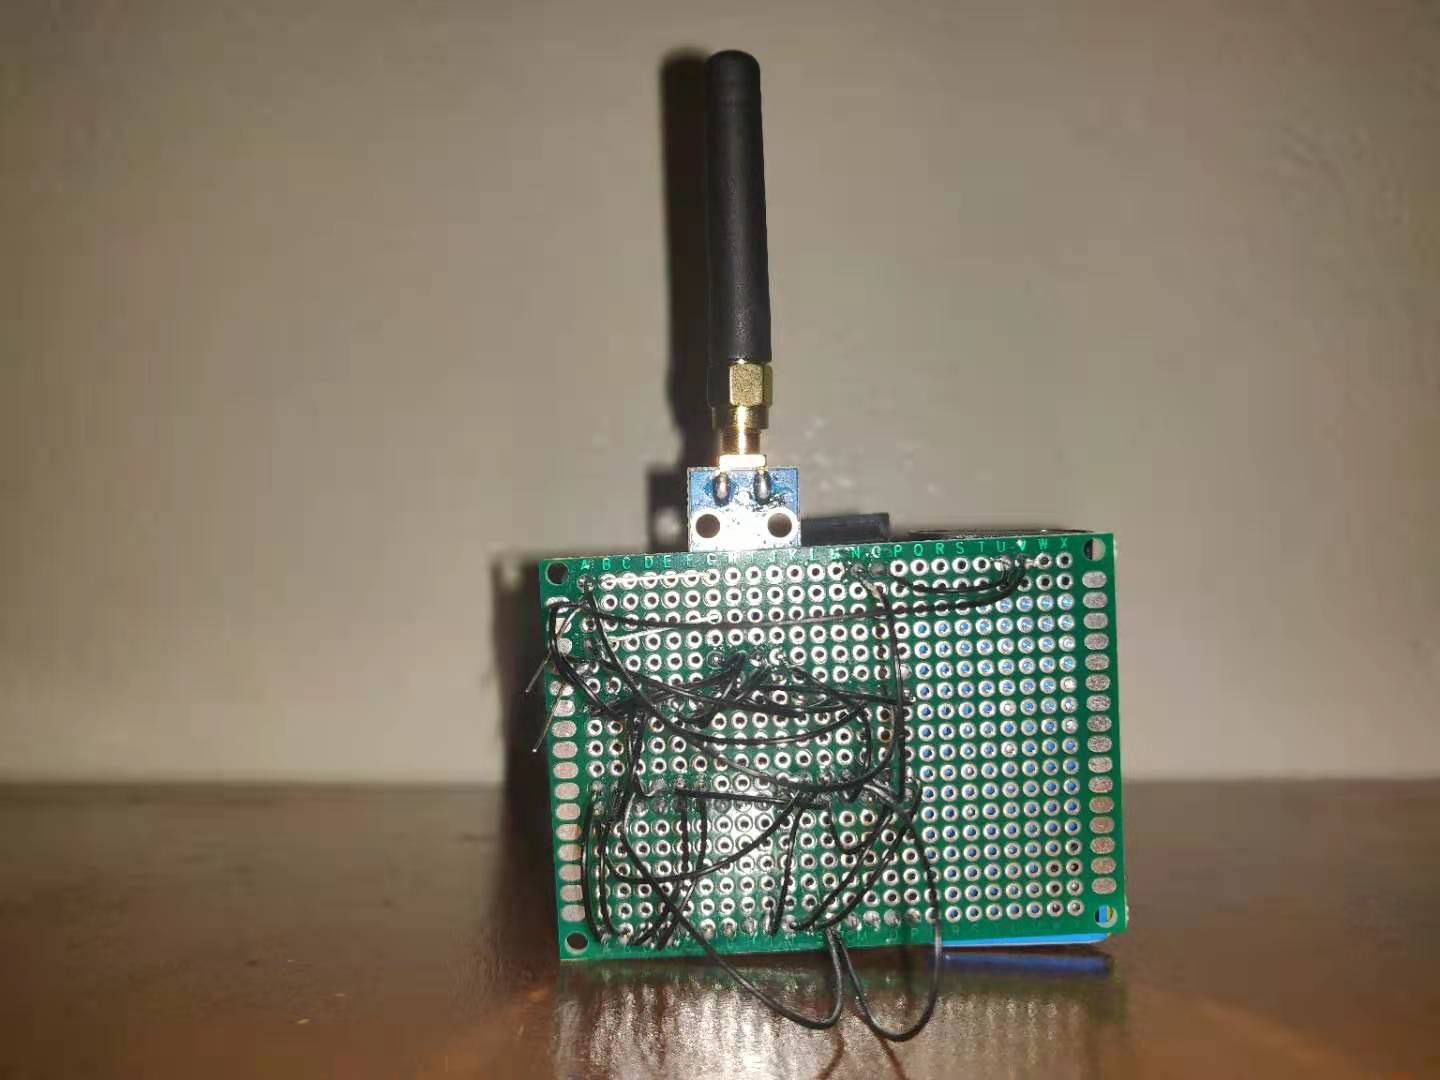
\includegraphics[width=6cm]{figures/prototype_back.jpg} }}%
    \caption{CR Device Prototype}%
    \label{fig:prototype_front_back_view}%
\end{figure}

One challenge putting together the components on the prototype board is the hand soldering part. All the components can be found on the front side of the board panel, while the wiring is hiding at the back panel. Each slot that needs to be soldered - most of these slots are big nodes - have two or three wires going into them. With the header pin that plugs from the front through the back, it may be  difficult for the single node to accommodate all wires during the soldering process. To avoid shorting at the crossing wire, the wires are conductive material with plastic insulators around it. The metal only exposes about 5mm towards both ends. The headers are placed at the designated prototype pin holes. Taking the height of the components into consideration, the orientation of the headers must be accurate and straight in order to fit in this limited space. Inserting headers are extremely beneficial for this project in the long run. The board, headers, and wires arrange the interconnection of the device. Components such as Arduino Nano, levels shifters, battery, and transceiver can be plugged in to use. While certain hardware parts may fail, users can replace those hardware components without disassembling the whole board. When upgrading the prototype, all the components can be recycled and used for the next project. This method helps the devices' sustainability. For the Bill of Material of the full board, please refer to Table~\ref{tab:bill} in the Appendix.


\section{Verification}

This hardware design passes a series of functional unit-tests and fulfills all requirements for a CR testbed. Below are the physical confirmation of the component use cases and the test methods.

\begin{itemize}
  \item components I/O current conforms the specification\newline
  Method: Arduino Nano data sheet shows that 40 mA of current can be generated to drive other loads. 40 mA of driven current is well above the requirement of both the level-shifters and transceiver, which is shown in their data sheet.
  \item transmission stays stable within range\newline
  Method: They are tested with constant transmission and receiving functionality within ten minutes of operation duration and ten meter of ranges in room temperature.
  \item batteries are capable for running number of experiment runs.\newline
  Method: A 9 V battery is advertised to have 500 mAh charge capacity. It is capable of running for five or more hours.
\end{itemize}

Below are the list of behavioral confirmations of the system.

\begin{itemize}
  \item BS recognizes and identifies all types of devices\newline
  Method: Within the synchronization phase, the BS can receive the message from all devices with specific protocol and insert them into the ready-list. LED indicators from the BS flashes to confirm this process.
  \item LBU and CPE connect to BS \newline
  Method: LBU and CPE connect to the BS separately. LED indicators from LBU and the CPE flashes to confirm this process.
  \item LBU and CPE synchronize with BS\newline
  Method: After the synchronization process, all LED indicators flash at the same time as they begin the experiment.
  \item LBU reads its unique schedule from the \texttt{TEST} library and switches channels\newline
  Method: LBU transmits in designated channels at certain time periods that are specified in the \texttt{TEST} library.
  \item CPE recognizes the termination time\newline
  Method: CPE reads and compares current time and termination time defined in the \texttt{TEST} library. When they match, it will end the experiment.
  \item CPE records data to and output data from the \texttt{EEPROM}\newline
  Method: CPE can write to the \texttt{EEPROM} and read from the \texttt{EEPROM}. It is confirmed by a simple read and write program.
  \item CPE would delay prime number amount of time when receiving no response during requesting state\newline
  Method: During the requesting state, after the CPE sends out the message and timer expires, CPE will wait for the series list of prime number time delay to begin the next attempt.
  \item CPE senses if the channel is free or busy\newline
  Method: CPE immediately hops out of the assigned channel if LBU is already transmitting. During CPE transmission, it will hop back to the reserved channel if the LBU happens to intercept in the middle.
  \item BS detects LBU\newline
  Method: In the periodic sensing function, BS can detect the environment with the confirmation of the LED indicators.
  \item BS selects a valid channel\newline 
  Method: Experiment with LBUs occupying the specific channel causes BS to choose the specific one. 
  \item BS updates channel and client status\newline
  Method: BS prints out all the channel and client statuses at some simple test cases. It updates the status lists whenever there is a change.
  \item BS updates selection table\newline
  Method: BS prints out selection at some simple test cases. It updates the selection table and makes the best decision.
\end{itemize}



\chapter{Systematic Experiment}
\section{Setup}

This chapter demonstrates how the testbed can be utilized in a specific scenario. First of all, the testbed requires users to define all the test cases in the \texttt{TEST} library. With the library, during the program uploading process, the specific device software would read the library and obtain some initial conditions much easier. Inside that library, users are supposed to construct schedule-lists for LBUs, and potentially action-lists for customized CPE behaviors. Both time division and end time should also be specified inside the library header file. The conditions of the spectrum, such as the number of the channel, the number of CPEs and LBUs in the test, should be specified in the \texttt{TEST} library as well. The testbed demonstration is designed to test with 1 BS, 5 CPEs, 3 LBUs to establish a single network region. The test will run for 1 week in virtual time, which translates to 15 minutes in real time.

Next, after setting up the testing stimulus, users should make sure the constant - ``operation'' = ``1'', running the experiment, in each of the programs: \texttt{base\_station.ino}, \texttt{customer\_premises\_equipment.ino} or \texttt{licensed\_band\_user.ino}. Then, the programs are ready to be uploaded to the relevant devices. The project suggests that users use Arduino IDE to compile and upload all of the code. During the uploading process of LBUs and CPEs, even though each of these devices may need the same process code, it is important to assign unique ID names to them. Before uploading each one of LBUs and CPEs, be sure to change the ID that is located at the top of the ``.ino'' files. After all the uploadings, the devices will be ready to be launched. 

Before running the experiment, picking a location for the experiment is very important. All devices should be able to ``see'' each other at a distance, especially the BS. Try to find an open space where there is not much signal interference around the network operating frequency range. The demonstration that this paper explores picks an indoor location with each device separated two to three meters apart. The BS is located at the center of the region, and all the rest of the devices would just make a circle around it with a radius of approximately three meters. After the placement, a pre-test shows that they can clearly transmit or receive data from each other. This concludes the setup portion of the testbed experiment.

\section{Operation}

To begin the test, users need to turn on the devices one by one. First start with the BS, then the CPEs, and lastly the LBUs. For each CPE or LBU that is turned on, its blue LED will  first turn on and then off indicating a connection setup request has been sent into the air. The BS catches the connection request, responds to it and stores the corresponding client ID in the client-list. The blue LED from the CPE will turn on and stay on, indicating it is in ready state after receiving the response from the BS. If the blue LED turns off and stays off for a long time, that shows the initial connection has not been successfully established. In this case, this is probably due to weak signals in the area. Users should check the battery and try changing the location of the device. Then, simply launch the device to establish the connection again. The LBU connection process is the same as the one for CPE. The launching order doesn't matter within the same type of device. After the last LBU receives the connection indication, the BS should recognize that all devices are ready for the experiment. The BS will broadcast a ``start'' message to the air, so that every device receives and starts the program at the same time. All CPEs and LBUs turn off their lights at the same time, indicating they have received the broadcast at the same time. This is the initial synchronization process for the testbed.

During the experiment, the LEDs from the CPE flash, showing that the experiment is running perfectly. The demonstration runs for approximately 15 minutes. Within the time, one CPE may have a blue light on and the other CPE may have a yellow light on. This means the CPE with the blue light on is sending data to the CPE with yellow light on in a certain channel. The communication will go on for 5 seconds since the time division was set to 5 seconds for this demonstration. Sometimes the LEDs for a pair of communicating CPEs will suddenly black out during the 5 seconds. This is because the communication is interrupted by a LBU. After the communication is done, lights from the CPEs would also be turned off as they both go back to the requesting state. While all the successful communications and interruptions happen during the experiment, the occurrence counts are actually recorded by each individual CPEs. 

To output the result from the memory,the CPEs have to be given the memory outputting code. Simply change the defined variable ``operation'' to 2 at the beginning of the \texttt{customer\_premises\_equipment.ino} file and upload to the CPE devices. As the device is turned on, it will run the memory outputting code. The Serial Monitor tool in Arduino IDE communicates with the device through SPI. When the individual device is connected to a client machine through USB, Arduino IDE can extract all the data inside Arduino EEPROM and print it to screen. Users can store the data for further process. If the experiment contains more than one trial, store the data this way after every trail, since the data would be erased and replaced by the new value from the next trial. This is what the operation process would look like. 


\section{Result and Discussion}

Determining if the testbed is a feasible tool for some of the algorithms out there could be broken down into the following ways: examining if the system operates normally and seeing if the output data expresses analytical value. The demonstration experiment mentioned in this chapter is designed to meet the two evaluation schemes. The same setup and operation runs four times, three with constant communication duration time, the other one with random communication duration time. Within the first three trials, they use different channel selection methods: first is in-order, second is random, third is with selection table. 

An hypothesis is made by taking consideration of the previous related project works. Before the testbed, the thesis project, there are two software simulations with different objectives launched for senior project. The first project was implemented in MATLAB Simulink to simulate CR channel switching mechanism in a hardware environment. See Figure~\ref{fig:top_level_simulink} and Figure~\ref{fig:random_signal_simulink} in the Appendix for the detailed setup. It drew the conclusion of switching times has an exponential relationship with the channel busy rate. However, in the other project, it tries to implement Python code to simulate and resolve the issue by trying a smarter channel selection algorithm. See Appendix for part of the code. It is also available in GitHub
https://github.com/SaltFishBoi/cognitive\_radio\_network\_simulator

The result shows, to a certain extent, it reduces channel switching time. If it is integrate to a physical environment, the results should be coincided.

Thus, methodology of the test relies on the assumption that channel switching is heavily affecting the performance of the system. With this assumption, there should be a linear relationship between performance and interruption count because each interruption requires a handoff or a channel switching, referring to the Figure~\ref{fig:channel_hopping}. When there are less interruptions, it implies that the network is utilizing the spectrum very well. Similarly, the more successful communication counts there are at the end of a trial, the better the algorithm it has. Therefore, the testbed is capable of accumulating the interruption counts, as well as the successful communication counts.

\begin{figure}[ht]
\centering
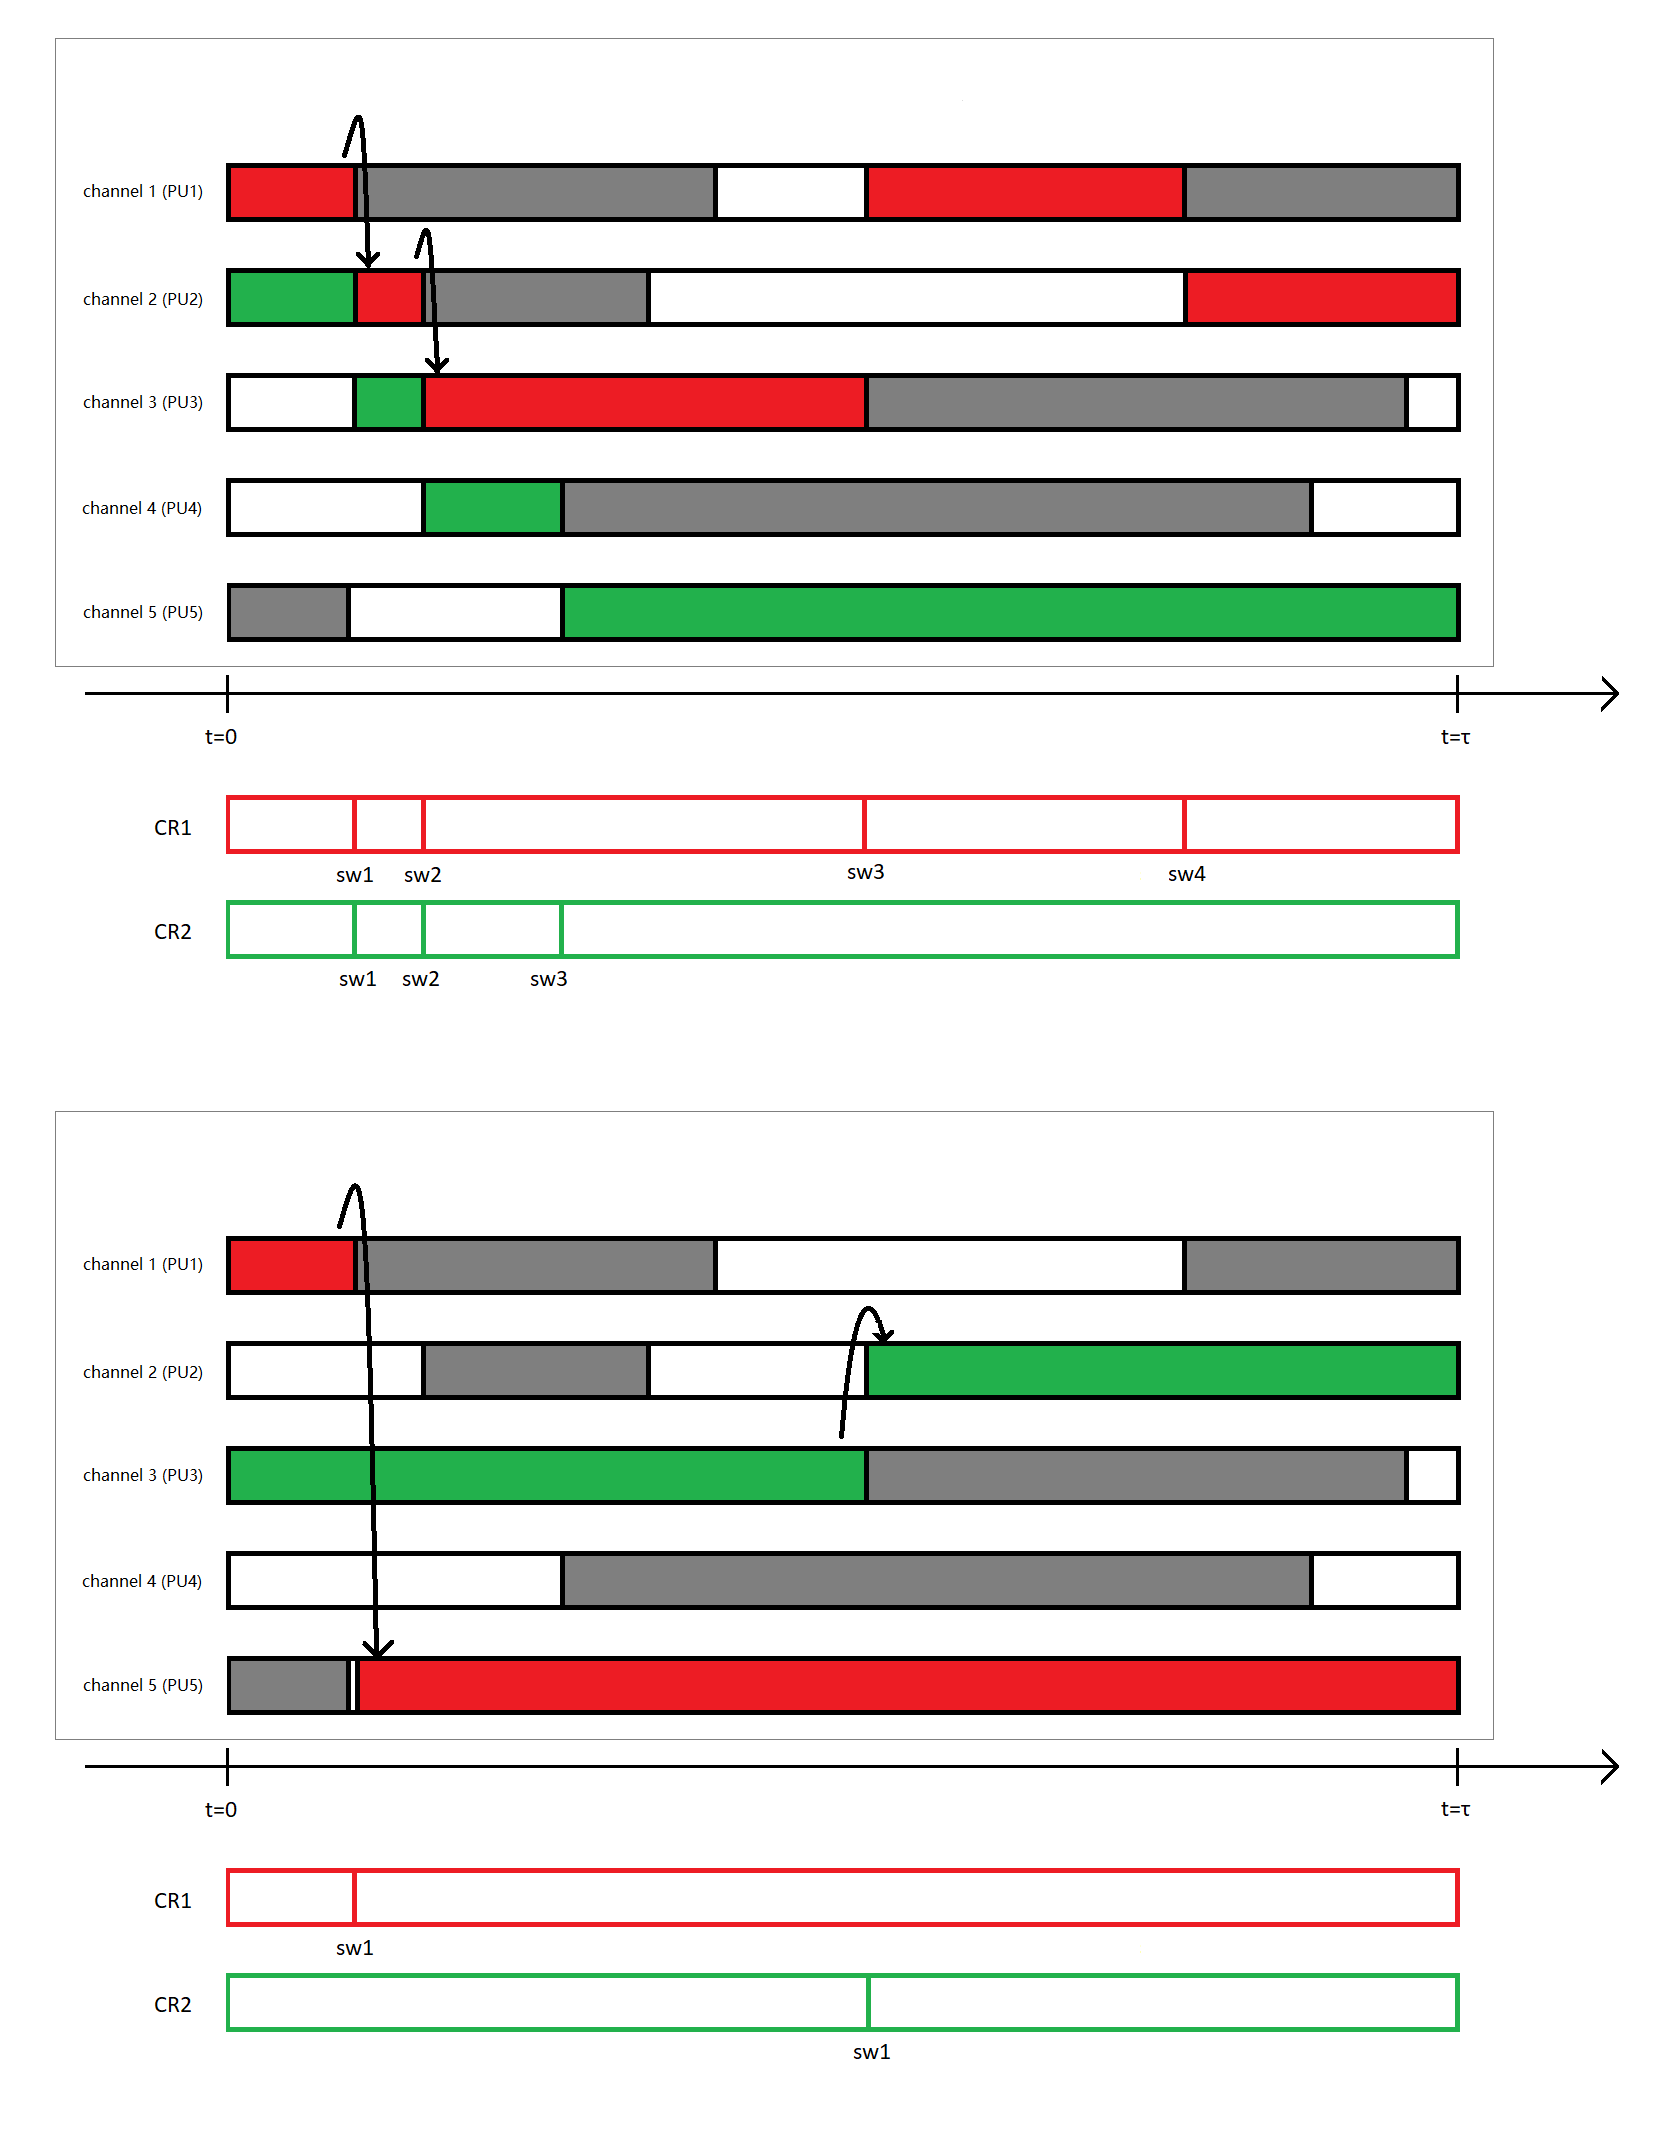
\includegraphics[width=10cm]{figures/channel_hopping.png}
\caption{Channel Hopping Comparison}
\label{fig:channel_hopping}
\end{figure}

The results show some interesting trends when comparing different channel selection algorithms and conditions. First, the comparison is represented in a bar graph shown in Figure~\ref{fig:performance_with_different_methods}. Here, it shows a graph of total transmission count across the same duration versus different channel selection choices. When using in-order selection, there are 131 transmissions without interruption within the 15 minutes of the trial. As it switches to random selection, a 140 success count is recorded. They have less than 10 percent of differences between the short 15 minutes. In theory, when the test stimulus signifies stochastic cases, there should not be any difference in choosing between the above two selection methods. Thus, the minor difference shown in the success transmission counts does not exemplify one method is superior than the other. However, the last trial has a significance of a 233 success transmission counts; it is approximately 60 percent more counts than the others. By simply adding a historical table or a selection table that keeps track of the spectrum usage, the system has a 1.6 times greater performance than the na\"ive logics. Figure~\ref{fig:interruption_in_a_week}(a) also illustrates a detailed interruption counts across the period of seven days in the trial. In-order and random channel selection methods shows a uniformly distributed data across the days. Yet, with the selection table inserted in the system, it shows trends of self-recognizing and self-learning during the process. After the first day with a lot of interruptions, it adapts and minimizes the interruptions, which is the key to maintain a high success transmission rate. In theory, since the test stimulus is designed to repeat every day, after the initial day, the system with historical data would have zero interruption for the rest of the time. Reasons for this remaining occurrence of interruption are both contributed by imperfection in the system logic and information delay during the update. With the result and knowledge of the system, users can have a rough evaluation of a channel selection algorithm.


\begin{figure}[ht]
\centering
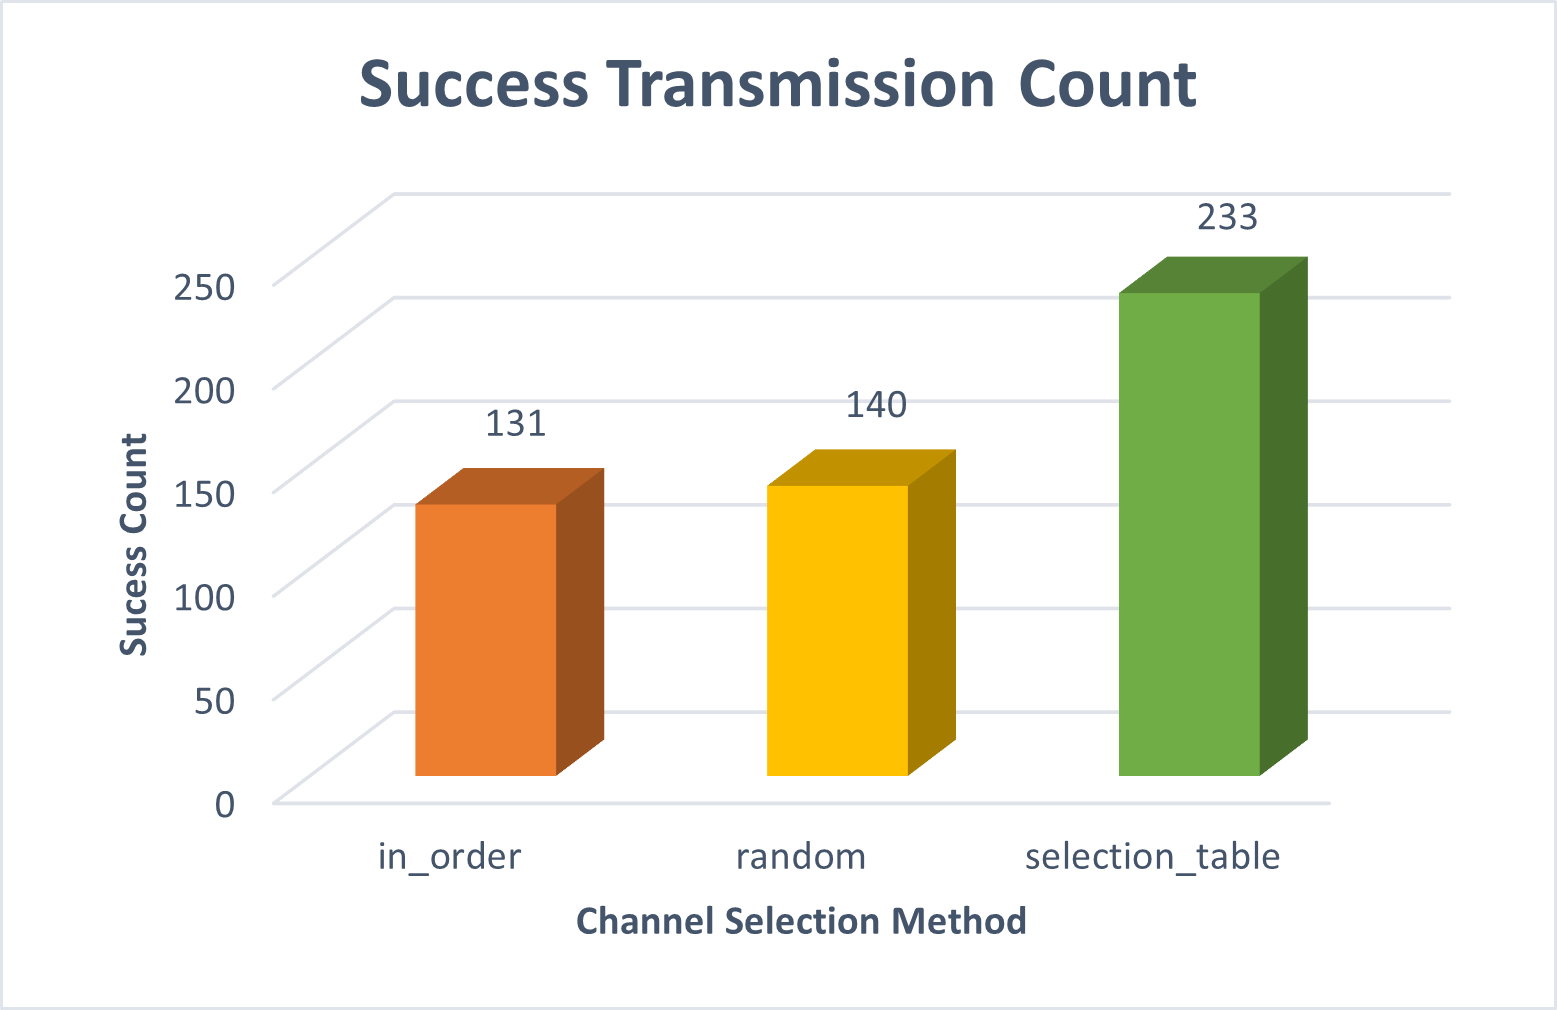
\includegraphics[width=10cm]{figures/total_success_count.png}
\caption{Over all Performance between Different Selection Methods}
\label{fig:performance_with_different_methods}
\end{figure}

Then, to push the system with the selection table further, another trial is set up to test its capability to adapt to varying transmission time of the devices. As it shows in Figure~\ref{fig:interruption_in_a_week}(b), the divergence of the interruption count is not as great as the system that has a predicted transmission time. Yet, it demonstrates the trend of self-learning during the process as well. This kind of environment is also more appropriate when describing a real-life communication process, associating with an unpredictable communication duration. To accommodate different objects and regulations, users can tune the testing environment accordingly. To a certain extent, this testbed does represent the potential value of a proposal CR algorithm.

\begin{figure}[ht]
  \subfloat[Comparing Behavior with Different Selection]{
	\begin{minipage}[c][0.7\width]{
	   0.4\textwidth}
	   \centering
	   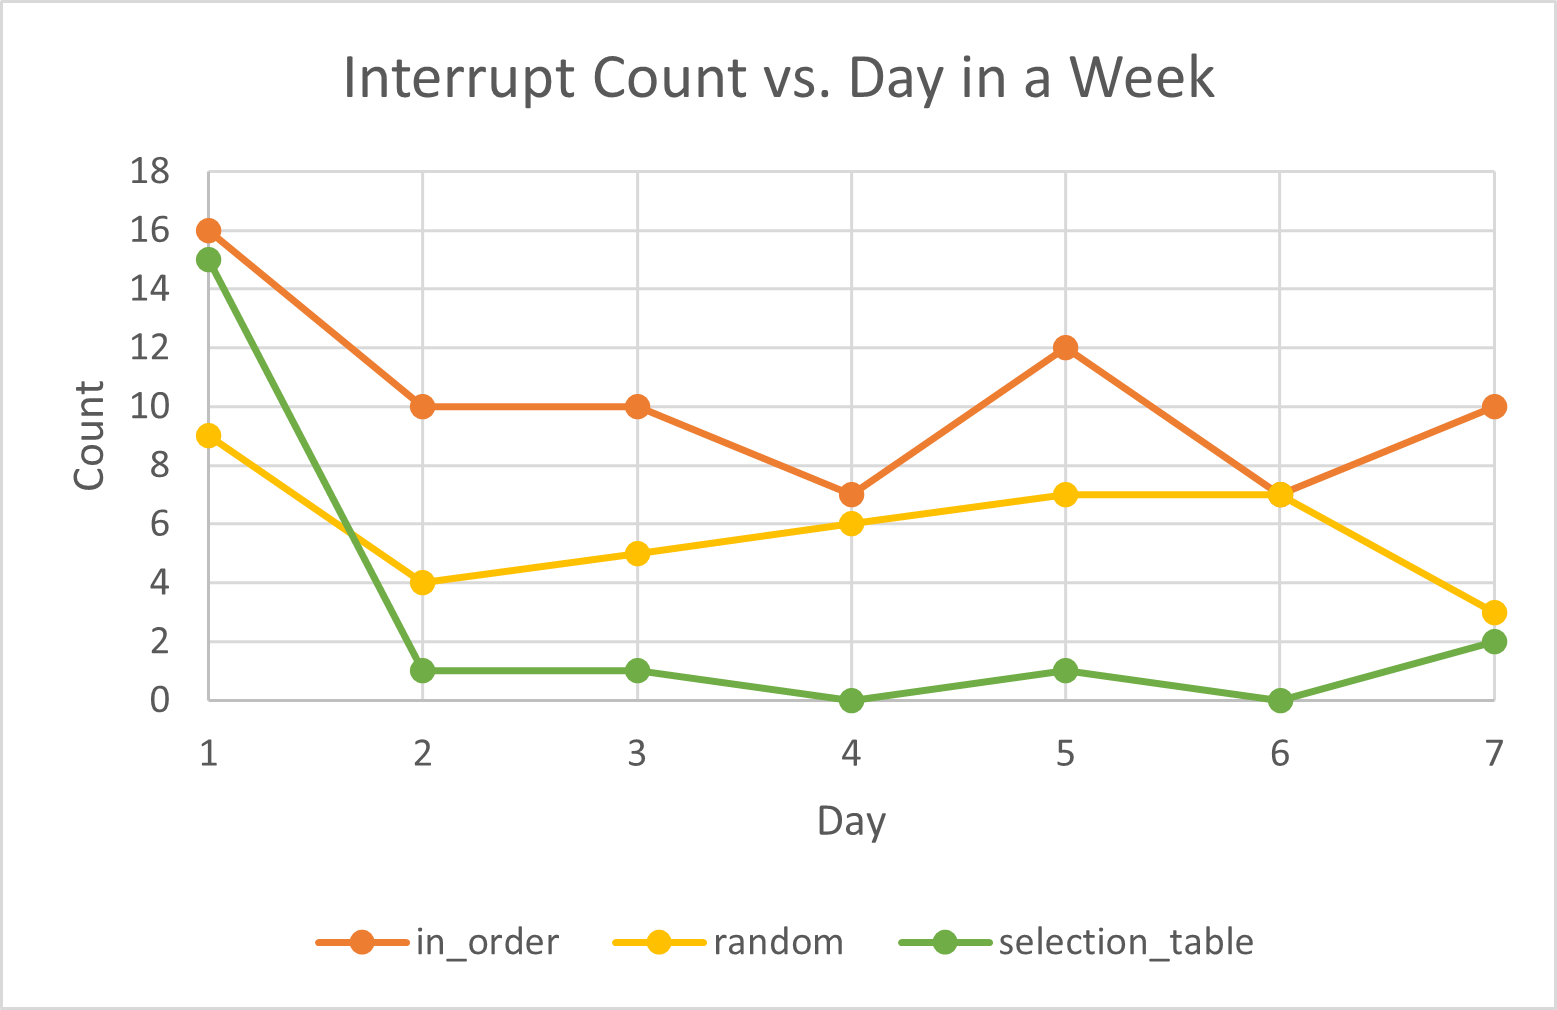
\includegraphics[width=1\textwidth]{figures/selection_comparison.png}
	\end{minipage}}
 \hfill 	
  \subfloat[Comparing Behavior with Different Duration Setup]{
	\begin{minipage}[c][0.7\width]{
	   0.4\textwidth}
	   \centering
	   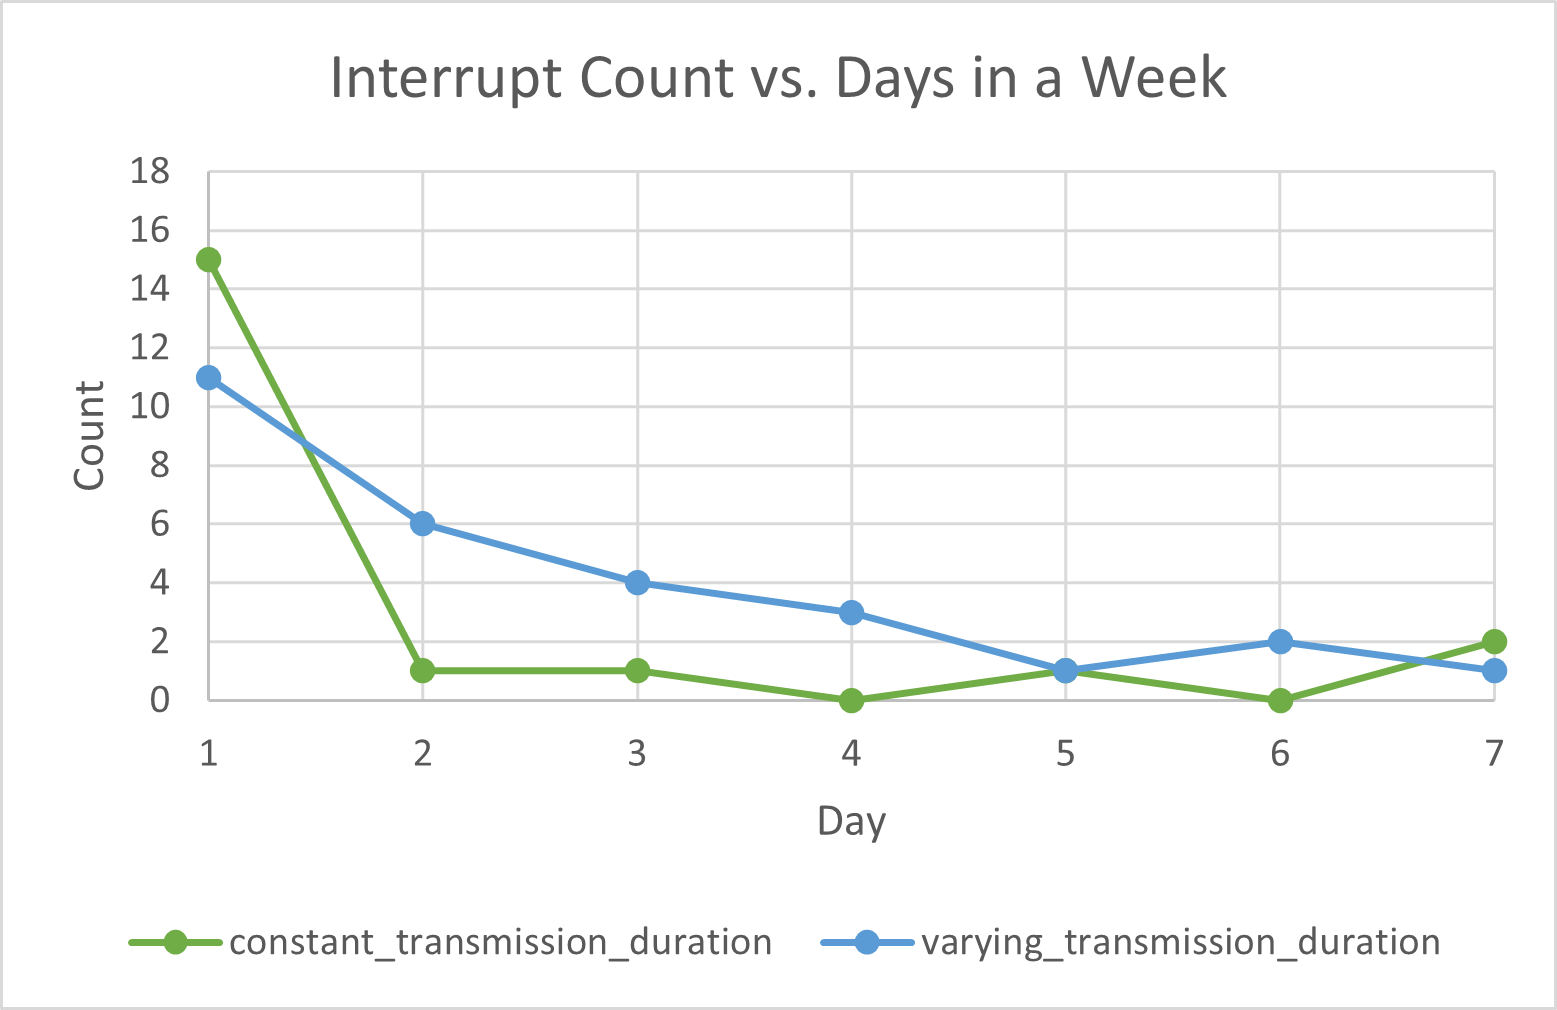
\includegraphics[width=1\textwidth]{figures/duration_comparison.png}
	\end{minipage}}
\caption{Interruption Counts across the Seven Days in a Week}
\label{fig:interruption_in_a_week}
\end{figure}





\chapter{Conclusion}
\section{Future Work}
Take note that the current testbed contains limitations. It accommodates basic regulation of an operating radio device, however, a set of much detailed and rigorous rules must be integrated into the system for commercial or military uses. The testbed is built around the CR algorithm proposals under the field of reactive channel selection. Area such as proactive channel selection requires another platform to keep all the spectrum data for regional networks to access. This requires a setup of a designated, centralized data division to process spectrum history. With a proactive channel selection system, the focus will be minimizing the channel switching delay of the hardware. Speaking of sharing knowledge from a region to another, simply adding more BSs can accomplish some of that. This takes it to the next level of cognitive radio network, which allows any sequential CR project launch to adopt the system very easily. Another aspect of the study, geo-barrier during employment, is also very important. Each device would not only be capable of recognizing other devices, they must also need to analyze the signal strength and advise the user for a better location. That is where city planning or location management comes into place. Looking back to the hardware, in fact, all should take this thesis project as purely a model of the system. The end goal for this system is to fully integrate onto a printed circuit board. These could be continually worked on and refined in the near future. 

\section{Summary}
In conclusion, this project integrates selective standards and guidelines that are given to form a CRN into a scalable testbed for future studies. The information gathered is initially around CR technology itself. To establish a network, it involves some basic protocol and radio frequency knowledge. Making a physical testbed, it is necessary to go through the whole hardware development and verification process. The experiments run in the testbed results in emulated data, which reflects the performance of certain CR logic. 

Now, with the understanding of where the CRN will be directed, all should stay tuned to this technology. Soon it may be implemented in our local network before you know it.


\nocite{*}
\bibliography{bibliography}

% Indents Appendix in Table of Contents
\makeatletter
\addtocontents{toc}{\let\protect\l@chapter\protect\l@section}
\makeatother

% Hack to make Appendices to appear in Table of Contents
\addtocontents{toc}{%
   \noindent APPENDICES
}
\begin{appendices}
\chapter{Function}
\begin{table}[ht]
\centering
    \begin{tabular}{ | l | p{5.5cm} | p{5cm} |}
    \hline
    Function  & File Use & Summary \\ \hline
    \texttt{millis} & \texttt{RADIO} \newline
    \texttt{base\_station} \texttt{customer\_premise\_equipment} \texttt{licensed\_band\_user} & extracts current time based on internal clock. \\ \hline
    \texttt{random} & \texttt{base\_station} & generates random integers for a given range. \\ \hline
    \texttt{delay} & \texttt{TEST} \newline
    \texttt{base\_station} \texttt{customer\_premise\_equipment} \texttt{licensed\_band\_user} & waits for a given time ms. \\\hline
    \texttt{digitalWrite} & \texttt{base\_station} \texttt{customer\_premise\_equipment} & sets a out put pin to a voltage value. \\\hline
    \texttt{pinMode} & \texttt{base\_station} \texttt{customer\_premise\_equipment} \texttt{licensed\_band\_user} & specifies digital GPIO usage.\\\hline
    \texttt{Serial.begin} & \texttt{base\_station} \texttt{customer\_premise\_equipment} \texttt{licensed\_band\_user} & initializes serial ports baud rate. \\\hline
    \texttt{Serial.print} & \texttt{base\_station} \texttt{customer\_premise\_equipment} \texttt{licensed\_band\_user} & output data to monitor through serial ports. \\\hline
    \hline
    \end{tabular}
\caption{Functions used from \texttt{Arduino}}
\label{tab:function}
\end{table}

\leavevmode\newline

\begin{table}[ht]
\centering
    \begin{tabular}{ | l | p{5.5cm} | p{6cm} |}
    \hline
    Function  & File Use & Summary \\ \hline
    \texttt{read} & \texttt{TEST} & reads the value in a given memory location. \\ \hline
    \texttt{write} & \texttt{TEST} & writes the value into a given memory location. \\ \hline
    \hline
    \end{tabular}
\caption{Functions used from \texttt{EEPROM}}
\label{tab:function2}
\end{table}

\leavevmode\newline

\begin{ThreePartTable}
\begin{TableNotes}
\footnotesize
\item Note: This table concludes all the functions used by \texttt{RADIO} to develop more handy subroutine for the system.
\end{TableNotes}
\begin{longtable}[ht]{ | l | p{10cm} | {c}}
\caption{Functions in \texttt{ELECHOUSE\_CC1101\_SRC\_DRV}}  \\
\hline
    Function & Summary \\ \hline
    \texttt{Init} & presets module registers. Each device must be set to initialize the cc1101. \\ \hline
    \texttt{setCCMode} & sets configuration for internal transmission mode. \\ \hline
    \texttt{setModulation} & sets modulation mode. 0 = 2-FSK, 1 = GFSK, 2 = ASK/OOK, 3 = 4-FSK, 4 = MSK. \\\hline
    \texttt{setMHz} & sets the basic frequency. The lib calculates the frequency automatically (default = 433.92).The cc1101 can: 300-348 MHZ, 387-464MHZ and 779-928MHZ. Read More info from datasheet. \\\hline
    \texttt{setDeviation} & sets the frequency deviation in kHz. Value from 1.58 to 380.85. Default is 47.60 kHz.\\\hline
    \texttt{setChannel} & sets the Channel number from 0 to 255. Default is channel 0. \\\hline
    \texttt{setChsp} & sets to multiply by the channel number CHAN and added to the base frequency in kHz. Value from 25.39 to 405.45. Default is 199.95 kHz. \\\hline
    \texttt{setRxBW} & sets the Receive Bandwidth in kHz. Value from 58.03 to 812.50. Default is 812.50 kHz. \\\hline
    \texttt{setDRate} & sets the Data Rate in kBaud. Value from 0.02 to 1621.83. Default is 99.97 kBaud. \\\hline
    \texttt{setPA} & sets TxPower. The following settings are possible depending on the frequency band.  (-30  -20  -15  -10  -6    0    5    7    10   11   12) Default is max! \\\hline
    \texttt{setSyncMode} & combines sync-word qualifier mode. 0 = No preamble/sync. 1 = 16 sync word bits detected. 2 = 16/16 sync word bits detected. 3 = 30/32 sync word bits detected. 4 = No preamble/sync, carrier-sense above threshold. 5 = 15/16 + carrier-sense above threshold. 6 = 16/16 + carrier-sense above threshold. 7 = 30/32 + carrier-sense above threshold. \\\hline
    \texttt{setSyncWord} & sets sync word. Must be the same for the transmitter and receiver. (Syncword high, Syncword low) \\\hline
    \texttt{setAdrChk} & controls address check configuration of received packages. 0 = No address check. 1 = Address check, no broadcast. 2 = Address check and 0 (0x00) broadcast. 3 = Address check and 0 (0x00) and 255 (0xFF) broadcast. \\\hline
    \texttt{setAddr} & modifies address used for packet filtration. Optional broadcast addresses are 0 (0x00) and 255 (0xFF). \\\hline
    \texttt{setWhiteData} & turns data whitening on / off. 0 = Whitening off. 1 = Whitening on. \\\hline
    \texttt{setPktFormat} & formats RX and TX data. 0 = Normal mode, use FIFOs for RX and TX. 1 = Synchronous serial mode, Data in on GDO0 and data out on either of the GDOx pins. 2 = Random TX mode; sends random data using PN9 generator. Used for test. Works as normal mode, setting 0 (00), in RX. 3 = Asynchronous serial mode, Data in on GDO0 and data out on either of the GDOx pins. \\\hline
    \texttt{setLengthConfig} & sets the length of message. 0 = Fixed packet length mode. 1 = Variable packet length mode. 2 = Infinite packet length mode. 3 = Reserved \\\hline
    \texttt{setPacketLength} & indicates the packet length when fixed packet length mode is enabled. If variable packet length mode is used, this value indicates the maximum packet length allowed. \\\hline
    \texttt{setCrc} & chooses CRC option. 1 = CRC calculation in TX and CRC check in RX enabled. 0 = CRC disabled for TX and RX. \\\hline
    \texttt{setCRC\_AF} & Enable automatic flush of RX FIFO when CRC is not OK. This requires that only one packet is in the RXIFIFO and that packet length is limited to the RX FIFO size. \\\hline
    \texttt{setDcFilterOff} & disables digital DC blocking filter before demodulator. Only for data rates less than or equal to 250 kBaud The recommended IF frequency changes when the DC blocking is disabled. 1 = Disable (current optimized). 0 = Enable (better sensitivity). \\\hline
    \texttt{setManchester} & enables Manchester encoding/decoding. 0 = Disable. 1 = Enable. \\\hline
    \texttt{setFEC} & enables Forward Error Correction (FEC) with interleaving for packet payload (Only supported for fixed packet length mode. 0 = Disable. 1 = Enable. \\\hline
    \texttt{setPQT} & sets the preamble quality estimator threshold. The preamble quality estimator increases an internal counter by one each time a bit is received that is different from the previous bit, and decreases the counter by 8 each time a bit is received that is the same as the last bit. A threshold of 4 PQT for this counter is used to gate sync word detection. When PQT=0 a sync word is always accepted. \\\hline
    \texttt{setAppendStatus} & enables status with two bytes be appended to the payload of the packet. The status bytes contain RSSI and LQI values, as well as CRC OK. \\\hline
    \texttt{CheckRxFifo} & checks if the receive flag is raised, buffer then ready to receive data\\\hline
    \texttt{CheckCRC} & uses cyclic redundancy check to ensure fullness of the data \\\hline
    \texttt{ReceiveData} & puts data to a buffer  \\\hline
    \texttt{SendData} & send data from the buffer to the air \\\hline
    \insertTableNotes  % tell LaTeX where to insert the contents of "TableNotes"
%\caption*{State Table for the proposed network (continued)}\\
\label{tab:function3}
\end{longtable}
\end{ThreePartTable}

\begin{table}[ht]
\centering
    \begin{tabular}{ | l | l | l | l | l | p{4cm} |}
    \hline
    Operation & opcode & payload & src & dest & Summary \\ \hline
    cpeRequest & 1 & T$^a$  & requester$^b$  & receiver$^c$ & sends whenever the requesting CPE wants to set up a connection with another CPE \\ \hline
    cpeRespond & 2 & CH$^d$ & receiver & requester & responds back to the requesting CPE by confirming the channel\\ \hline
    cpeSend & 3 & X$^e$ & receiver & requester & sends to the receiving CPE at the assigned channel \\ \hline
    bsRequest & 5 & CH & requester & receiver & forwards the message to the target CPE with BS selected channel\\ \hline
    bsRespond & 6 & CH & receiver & requester & forwards the response from the target CPE back to the requesting CPE\\ \hline
    cpeStart & 7 & X & requester & X & initiates the CPE initial connection to the BS\\ \hline
    lbuInterrupt & 8 & X & X & X & sends to interrupt the CPE communications \\ \hline
    lbuStart & 11 & X & requester & X & initiates the LBU initial connection to the BS \\ \hline
    bsStart & 12 & X & X & X & broadcasts to finish the synchronization process\\ \hline
    \hline
    \end{tabular}
\footnotesize{
$^a$ The varying communication time duration \
$^b$ The device that initiates the connection 
$^c$ The device that would catch the message 
$^e$ The assigned channel 
$^e$ Representation of a Don't Care value}\\
\caption{Message structure}
\label{tab:structure}
\end{table}


\chapter{Specification}

\begin{table}[ht]
\centering
    \begin{tabular}{ | p{5cm} | p{8cm} |}
    \hline
    Microcontroller & ATmega328\\ \hline
    Architecture & AVR\\ \hline
    Operating Voltage & 5 V\\ \hline
    Flash Memory & 32 KB of which 2 KB used by bootloader\\ \hline
    SRAM & 2 KB\\ \hline
    Clock Speed & 16 MHz\\ \hline
    Analog IN Pins & 8\\ \hline
    EEPROM & 1 KB\\ \hline
    DC Current per I/O Pins & 40 mA (I/O Pins)\\ \hline
    Input Voltage & 7-12 V\\ \hline
    Digital I/O Pins & 22 (6 of which are PWM)\\ \hline
    PWM Output & 6\\ \hline
    Power Consumption & 19 mA\\ \hline
    PCB Size & 18 x 45 mm\\ \hline
    Weight & 7 g\\ \hline
    Product Code & A000005\\ \hline
    \hline
    \end{tabular}
\caption{Arduino Nano Specification}
\label{tab:arduino_spec} \cite{arduino_nano}
\end{table}

\begin{table}[ht]
\centering
    \begin{tabular}{ | p{2cm} | p{5cm} | p{7cm} |}
    \hline
    No. & Parameter item & Parameter details and description\\ \hline
    1 & Size & 15 * 30mm\\ \hline
    2 & Components & Imported from Japan, USA and Germany\\ \hline
    3 & Connector & 2*4*2.54mm\\ \hline
    4 & Supply voltage & 1.9 - 3.6V DC (Notes: the voltage higher than 3.6V is forbidden.)\\ \hline
    5 & Frequency Band & 387 - 464MHz, adjustable, Recommending frequency: 433±10MHz\\ \hline
    6 & Communication level & 0.7VCC - 3.6V (VCC refers to the supply voltage)\\ \hline
    7 & Operation Range & About 520m(test condition: clear and open area and maximum power, antenna gain: 5dBi, height: $>$ 2m, air date rate:     1.2Kbps)\\ \hline
    8 & Transmitting power & Maximum 10dbm (10mW)\\ \hline
    9 & Air data rate & 0.6k - 500k(1.2~20kbps is recommended)\\ \hline
    10 & Sleep current & 0.6uA\\ \hline
    11 & Transmitting current & 29.2mA at 10dBm\\ \hline
    12 & Receiving current & 16.0mA  \\ \hline
    13 & Communication interface & SPI (data rate: up to 10Mbps)\\ \hline
    14 & Transmitting length & 1 - 64 bytes for one package\\ \hline
    15 & Receiving length & 1 - 64 bytes for one package\\ \hline
    16 & RSSI support & usable\\ \hline
    17 & Antenna type & SMA-K(External thread hole, 50 ohm impedance)\\ \hline
    18 & Sensitivity & -116dBm at 0.6kbps, -112dBm at 1.2kbps\\ \hline
    19 & Operating temperature & -40 \textasciitilde +85\textdegree{}C \\ \hline
    20 & Operating humidity & 10\% ~ 90\%\\ \hline
    21 & Storage temperature & -40 \textasciitilde +125\textdegree{}C \\ \hline
    \hline
    \end{tabular}
\caption{CC1101 Module Specification}
\label{tab:cc1101_spec}\cite{cc1101_module}
\end{table}


\chapter{Bill Of Material}
\begin{table}[h]
\centering
    \begin{tabular}{| l | l | l | c | r | }
    \hline
    Item & Description & Quantity & Units & Cost \\ 
    \hline
    \rowcolor{lightgray} Arduino Nano & MCU ATmega328 & 1 &  Dozen &  50.16 \\ 
    Arduino Adaptor  &  3.0 USB to mini USB & 1 &  Each &  0.64 \\ 
    \rowcolor{lightgray} Transceiver Module & E07-M1101D Board V2.0 & 1 &  Dozen &  33.6 \\ 
    Level Shifter &  pack of 10 & 2 &  Package & 13.98 \\ 
    \rowcolor{lightgray} Pin Header Socket &  16, 6 and 4 pins, pack of 10 & 12 &  Package &  5.76 \\ 
    Prototype Board & 5 x 7cm, pack of 10 & 1 &  Package &  4 \\ 
    \rowcolor{lightgray} Battery & 9V & 10 & Each &  1 \\ 
    Battery Connector &  T type Battery Connector & 1 & Dozen & 1.3 \\ 
    \rowcolor{lightgray} Light-emitting Diode &  blue and yellow & 20 &  Each &  1.04 \\ 
    Wire &  3m roll & 2 & Each &  1 \\ 
    \rowcolor{lightgray} Solder &  solder wire roll, 50g, 1mm & 3 &  Each &  1.71 \\ 
    \hline
    \hline
    \end{tabular}
    \begin{tablenotes}
    \small
    \item Note: The necessary tools such as the IDE accessible client machine or soldering iron are not included here.
\end{tablenotes}
\caption{Bill of Material}
\label{tab:bill}
\end{table}

\chapter{Simulink}
\begin{figure}[ht]
\centering
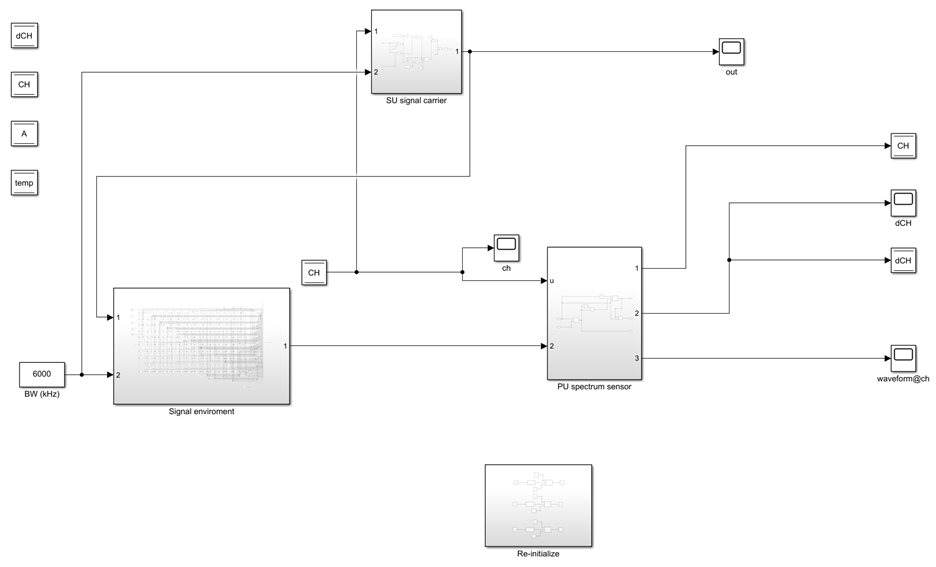
\includegraphics[width=12cm]{figures/top_level_simulink.png}
\caption{Top Level Block}
\label{fig:top_level_simulink}
\end{figure}

\begin{figure}[ht]
\centering
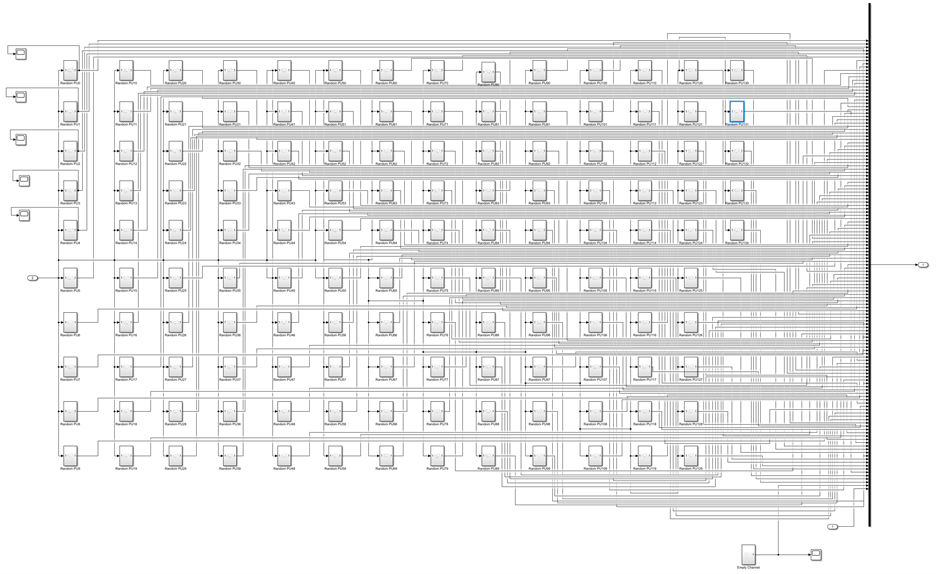
\includegraphics[width=12cm]{figures/random_signal_simulink.png}
\caption{Random Signal Generator Block}
\label{fig:random_signal_simulink}
\end{figure}

\chapter{Python Simulation}
\begin{lstlisting}[caption={Selected main process code in Python simulation},captionpos=b]
# Available at
# https://github.com/SaltFishBoi/cognitive_radio_network_simulator 
from base_station import *
from customer_premise_equipment import *
from licensed_band_user import *
from transmission import *
from algorithm import *
from multiprocessing import Process
import time

INTERRUPT_FLAG = 0

def main():

    # initialize environment channel list
    share_env1 = create_environment()

    # initialize base station
    bs = BS(0)

    # CPE action list
    # actions list (EDITABLE)
    # (delay, target)
    action_list = [[ACTION(1, 1, 10), ACTION(1, 11, 10)],
                   [ACTION(2, 2, 10), ACTION(2, 12, 10)],
                   [ACTION(3, 3, 10), ACTION(3, 13, 10)],
                   [ACTION(4, 4, 10), ACTION(4, 14, 10)],
                   [ACTION(5, 5, 10), ACTION(5, 15, 10)],
                   [ACTION(6, 6, 10), ACTION(6, 16, 10)],
                   [ACTION(1, 7, 10), ACTION(1, 17, 10)]]

    schedule_list = [[6, 6, 7, 8, 9],
                     [6, 6, 7, 8, 9],
                     [6, 6, 7, 8, 9],
                     [6, 6, 7, 8, 9],
                     [6, 6, 7, 8, 9],
                     [6, 6, 7, 8, 9],
                     [6, 6, 7, 8, 9],
                     [6, 6, 7, 8, 9],
                     [6, 6, 7, 8, 9],
                     [6, 6, 7, 8, 9],
                     [6, 6, 7, 8, 9]]

    print("Program Starts")

    # launch multiprocess

    t = Process(target=timing)
    t.start()

    b = Process(target=bs_process, args=(share_env1, bs))
    print("Program runs")
    cpe_proc = []
    lbu_proc = []
    b.start()

    # initialize and launch license band user list
    for i in range(1, NUM_LBU_DEFAULT+1):
        device = LBU(i, STATE_DEFAULT, i)
        l = Process(target=lbu_process, args=(share_env1, i, device, schedule_list[i-1]))
        l.start()
        lbu_proc.append(l)

    # initialize and launch customer premise equipment list
    for i in range(NUM_CPE_DEFAULT):
        device = CPE(i)
        c = Process(target=cpe_process, args=(share_env1, i, device, action_list[i]))
        c.start()
        cpe_proc.append(c)

    # recycle all processes
    for c in cpe_proc:
        c.join()

    for l in lbu_proc:
        l.join()

    b.join()
    t.join()
    print("Program ends")

    return 0

def timing():
    i = 0
    while True:
        print("    Time: ", i)
        time.sleep(1)
        i += 1
        
# Press the green button in the gutter to run the script.
if __name__ == '__main__':
    #stdoutOrigin = sys.stdout
    #sys.stdout = open("log.txt", "w")
    main()
\end{lstlisting}




\end{appendices}

\end{document}
